% !TEX program = xelatex
\documentclass[UTF8,fontset=none,a4paper,10pt]{ctexart}
\usepackage[a4paper,left=19mm,right=19mm,top=18mm,bottom=19mm,headheight=14pt]{geometry}
\usepackage{fontspec}
\setmainfont[
  BoldFont=texgyretermes-bold.otf,
  ItalicFont=texgyretermes-italic.otf,
  BoldItalicFont=texgyretermes-bolditalic.otf
]{texgyretermes-regular.otf}
\setsansfont[
  BoldFont=texgyreheros-bold.otf,
  ItalicFont=texgyreheros-italic.otf,
  BoldItalicFont=texgyreheros-bolditalic.otf
]{texgyreheros-regular.otf}
\setmonofont[
  BoldFont=texgyrecursor-bold.otf,
  ItalicFont=texgyrecursor-italic.otf,
  BoldItalicFont=texgyrecursor-bolditalic.otf,
  Scale=MatchLowercase
]{texgyrecursor-regular.otf}
\usepackage{amsmath,amssymb,booktabs,array,tabularx,longtable,multirow}
\usepackage{graphicx,xcolor,enumitem,float,caption,subcaption}
\usepackage{titlesec,fancyhdr,microtype,indentfirst}
\usepackage{tikz}
\usetikzlibrary{arrows.meta,positioning,fit,calc,backgrounds,shapes.geometric}
\usepackage{algorithm}
\usepackage{algpseudocode}
\usepackage[numbers,sort&compress]{natbib}
\usepackage{hyperref}
\usepackage{bookmark}
\renewcommand{\abstractname}{Abstract}
\renewcommand{\contentsname}{Contents}
\renewcommand{\figurename}{Figure}
\renewcommand{\tablename}{Table}
\renewcommand{\refname}{References}
\renewcommand{\appendixname}{Appendix}
\definecolor{navy}{HTML}{17365D}
\definecolor{linkblue}{HTML}{2459A6}
\definecolor{lightblue}{HTML}{EAF1FB}
\hypersetup{colorlinks=true,linkcolor=linkblue,citecolor=linkblue,urlcolor=linkblue,bookmarksnumbered=true,pdftitle={Understanding GPT-Live: A Public-Evidence-Based Architectural Reconstruction and Implementation Hypothesis},pdfauthor={Jiguo Li},pdfsubject={Technologies for Full-Duplex Continuous Inference Architectures}}
\microtypesetup{protrusion=true,expansion=false}
\linespread{1.13}
\setlength{\parindent}{2em}
\setlength{\parskip}{2.5pt}
\setlength{\abovedisplayskip}{6pt}
\setlength{\belowdisplayskip}{6pt}
\setlength{\abovedisplayshortskip}{4pt}
\setlength{\belowdisplayshortskip}{4pt}
\setlength{\jot}{3pt}
\emergencystretch=2em
\setlength{\textfloatsep}{8pt plus 2pt minus 2pt}
\setlength{\floatsep}{7pt plus 2pt minus 2pt}
\setlength{\intextsep}{7pt plus 2pt minus 2pt}
\setlist[itemize]{leftmargin=1.8em,itemsep=1pt,topsep=2pt,parsep=0pt}
\setlist[enumerate]{leftmargin=2em,itemsep=1pt,topsep=2pt,parsep=0pt}
\captionsetup{font=small,labelfont=bf,skip=3pt}
\titleformat{\section}{\Large\bfseries\color{navy}}{\thesection}{0.7em}{}
\titleformat{\subsection}{\large\bfseries\color{navy}}{\thesubsection}{0.65em}{}
\titleformat{\paragraph}[runin]{\normalsize\bfseries}{}{0pt}{}
\titlespacing*{\section}{0pt}{14pt}{5pt}
\titlespacing*{\subsection}{0pt}{10pt}{3pt}
\titlespacing*{\paragraph}{0pt}{0.65ex plus 0.2ex}{0.45em}
\pagestyle{fancy}
\fancyhf{}
\fancyhead[L]{\small\color{gray}GPT-Live Architectural Reconstruction}
\fancyhead[R]{\small\color{gray}\leftmark}
\fancyfoot[C]{\small\thepage}
\renewcommand{\headrulewidth}{0.3pt}
\renewcommand{\footrulewidth}{0pt}
\definecolor{official}{HTML}{1F77B4}
\definecolor{public}{HTML}{2CA02C}
\definecolor{hypothesis}{HTML}{D97706}
\newcommand{\FOne}{\textcolor{official}{\textbf{[F1]}}}
\newcommand{\FTwo}{\textcolor{public}{\textbf{[F2]}}}
\newcommand{\Hyp}{\textcolor{hypothesis}{\textbf{[H]}}}
\newcommand{\model}[1]{\textsf{#1}}
\newcommand{\ms}{\,\mathrm{ms}}
\newcommand{\noteBox}[1]{%
  \begin{center}
  \fcolorbox{linkblue}{lightblue}{\parbox{0.93\linewidth}{#1}}
  \end{center}}
% TeX Live fonts available in arXiv's XeLaTeX environment.
\setCJKmainfont[AutoFakeBold=2,ItalicFont=gkai00mp.ttf]{gbsn00lp.ttf}
\setCJKsansfont[AutoFakeBold=2]{gbsn00lp.ttf}
\setCJKmonofont{gbsn00lp.ttf}
% Keep the English and Chinese tables of contents independent in one TeX job.
\makeatletter
\let\BilingualOriginalAddContentsLine\addcontentsline
\def\BilingualTocExtension{entoc}
\renewcommand{\addcontentsline}[3]{%
  \def\BilingualRequestedExtension{#1}%
  \def\BilingualStandardToc{toc}%
  \ifx\BilingualRequestedExtension\BilingualStandardToc
    \BilingualOriginalAddContentsLine{\BilingualTocExtension}{#2}{#3}%
  \else
    \BilingualOriginalAddContentsLine{#1}{#2}{#3}%
  \fi
}
\renewcommand{\tableofcontents}{%
  \section*{\contentsname
    \@mkboth{\MakeUppercase\contentsname}{\MakeUppercase\contentsname}}%
  \@starttoc{\BilingualTocExtension}%
}
\newcommand{\BilingualUseEnglishToc}{\gdef\BilingualTocExtension{entoc}}
\newcommand{\BilingualUseChineseToc}{\gdef\BilingualTocExtension{zhtoc}}
\def\BilingualAnchorPrefix{en}
\let\BilingualOriginalAppendix\appendix
\renewcommand{\appendix}{%
  \BilingualOriginalAppendix
  \renewcommand*{\theHsection}{\BilingualAnchorPrefix.appendix.\Alph{section}}%
}
\makeatother

\begin{document}
\renewcommand{\abstractname}{Abstract}
\renewcommand{\contentsname}{Contents}
\renewcommand{\figurename}{Figure}
\renewcommand{\tablename}{Table}
\renewcommand{\refname}{References}
\renewcommand{\appendixname}{Appendix}
\BilingualUseEnglishToc
\renewcommand*{\theHsection}{en.\arabic{section}}
\renewcommand*{\theHsubsection}{en.\arabic{section}.\arabic{subsection}}
\renewcommand*{\theHsubsubsection}{en.\arabic{section}.\arabic{subsection}.\arabic{subsubsection}}
\renewcommand*{\theHequation}{en.\arabic{equation}}
\renewcommand*{\theHfigure}{en.\arabic{figure}}
\renewcommand*{\theHtable}{en.\arabic{table}}
\gdef\BilingualAnchorPrefix{en}
\markboth{}{}
\pdfbookmark[0]{English Version}{bilingual.english}
\begin{center}
 {\zihao{2}\bfseries\color{navy} Understanding GPT-Live: A Public-Evidence-Based Architectural Reconstruction and Implementation Hypothesis}\par
  \vspace{4pt}
 {\zihao{3}\color{navy} Technologies for Full-Duplex Continuous Inference Architectures}\par
  \vspace{10pt}
 {\normalsize\textbf{Jiguo Li\footnote{This article was completed with the assistance of Codex.}}}\par
  \vspace{2pt}
  {\small\href{mailto:jiguolee@gmail.com}{jiguolee@gmail.com}}\par
  \vspace{2pt}
{\small August 2026}
\end{center}
\vspace{5pt}
\hrule

\begin{abstract}
At the time of writing, OpenAI has not released a complete technical report on GPT-Live, nor has it disclosed implementation details such as the model architecture, audio representation, training data, or training procedure. This article is therefore not a restatement of an official OpenAI technical report or of the system's internal implementation; it is a technical reconstruction and implementation hypothesis based on public evidence. The work was motivated by a recent OpenAI engineering blog that describes several system-level choices behind the transition from turn-based voice interaction to continuous inference, including asynchronous delegation, stateful instance handoff, and low-latency transport. Starting from those disclosed system boundaries, we combine OpenAI engineering material and system documentation, Internet Engineering Task Force protocol drafts, recent full-duplex speech-model research, and open-source implementations to derive a plausible but unverified reference architecture. Our central hypothesis is that reproducing the capabilities demonstrated by GPT-Live requires the coordination of four layers: a full-duplex interaction core, asynchronous delegation to deeper reasoning and tool-use models, stateful serving for long-lived sessions, and low-round-trip-time media transport. We formalize continuous inference and compare publicly documented approaches based on codec tokens, codec-free representations, dual-stream fusion, cross-attention, finite-state-machine control tokens, and explicit action channels. We further analyze training data, overlapping speech, interruption behavior, attention caches, context compaction, instance handoff, fault recovery, WebRTC, and WARP, before presenting an open-source implementation proposal, ablation plan, and evaluation framework. The cited papers and open-source projects demonstrate possible mechanisms; they do not establish that GPT-Live uses the same designs. The article explicitly separates official facts, mechanisms established in public literature, and inference-based reconstruction.

\noindent\textbf{Keywords:} GPT-Live; full-duplex speech model; continuous inference; speech-to-speech; real-time systems; WebRTC; stateful serving
\end{abstract}

\noteBox{\textbf{Key point:} GPT-Live is not merely an end-to-end speech-to-speech model. Its behavior depends on the coordination of a full-duplex interaction core, asynchronous cognition, stateful serving, and low-latency transport.}

\clearpage
\begingroup
\small
\setlength{\parskip}{0pt}
\linespread{1.02}\selectfont
\setcounter{tocdepth}{2}
\tableofcontents
\endgroup
\clearpage

\section{Problem Definition, Evidence Boundaries, and Evolution}

\subsection{Origin of research: Starting from an engineering blog of OpenAI}

The direct origin of this article is the engineering blog "How We Built a Realtime System for Responsive Voice AI in Six Months" \cite{en:openai2026continuous} published by OpenAI on August 3, 2026. Unlike product introductions that usually focus on feature demonstrations and evaluation results, this article starts from engineering implementation, explaining why the team abandoned the traditional speech architecture that relied on turn detectors, and how to redesign the inference, context management, and media delivery systems within six months. Several details disclosed in the blog particularly aroused my interest: the speech model can listen and speak at the same time; media frames are transmitted through independent fast paths; complex reasoning and tool calls are executed along another asynchronous path; long sessions remain continuous through background context compression and model instance switching; WARP and Instant Connect try to further shorten WebRTC\footnote{Web Real-Time Communication, Web Real-time communication technology stack for low-latency audio, video and data transmission between browsers or clients. } Connection establishment time.

This public information outlines the system outline of GPT-Live, but it also leaves a more worthy question: How does the full-duplex speech model continue to receive new input during generation? How does the model represent overlapping speech from both sides and interactive actions such as pauses, short responses, and interruptions? How to transfer context and results between fast interaction models and deep inference models? How can a stateful session that lasts for tens of minutes remain smooth under GPU scheduling, KV cache, network jitters, and instance failures?

This blog thus became the starting point for this article. This article does not reiterate its product functions, but uses the disclosed system boundaries as clues, combined with top conference papers, technical reports, open source implementations and network protocols in recent years, to try to restore a set of GPT-Live architecture that is technically self-consistent and evidence-traceable. In other words, what this article wants to answer is not just "What capabilities does GPT-Live have?" but "What problems do the model and system need to solve in order to realize these capabilities?"

\subsection{What This Article Explains}

"How GPT-Live is implemented" contains two confusing questions. One is the \emph{ model problem }: how to represent audio, how the user flow enters Transformer, and how the model predicts semantics, acoustics and interactive actions at the same time. The second is \emph{ system issue }: network jitter, continuous sessions, GPU inference time limit, KV cache, how complex inference and tool invocation work together without interrupting voice interaction. GPT-Live's public materials show that system issues are as important as model issues \cite{en:openai2026gptlive,en:openai2026continuous}. Therefore, this article studies "an online speech agent that can handle natural speech overlaps, accept interruptions at any time, provide continuous feedback, and perform background tasks" rather than an isolated model checkpoint.

The evidence adopts three levels of annotation: \FOne only comes from OpenAI official articles and system cards; \FTwo comes from peer-reviewed papers, author technical reports, open source code or standards; \Hyp is an architectural reconstruction constrained by multiple facts. In particular, it needs to be emphasized that OpenAI does not disclose the parameters, audio tokenizer, frame rate, attention connection method, number of training tokens, or cluster size of GPT-Live. Work such as Moshi and DuplexOmni can demonstrate that a mechanism is engineeringly feasible, but cannot prove that GPT-Live uses the same mechanism.

\subsection{Four Generations of Voice Interaction}

\paragraph{Cascading voice pipeline}
Traditional systems are connected in series with VAD/endpointing, ASR, text LLM and TTS\footnote{VAD: Voice Activity Detection, voice activity detection; ASR: Automatic Speech Recognition, automatic speech recognition; LLM: Large Language Model, large language model; TTS: Text-to-Speech, text-to-speech. }. Its advantages are that modules are observable, components are easy to replace, and the text tool ecosystem is mature; the problem is that errors accumulate layer by layer, rhythm and non-verbal signals are lost at the text bottleneck, and each round must wait for "the user to finish speaking." The total delay can be roughly written as
\begin{equation}
T_{\mathrm{cascade}}=T_{\mathrm{endpoint}}+T_{\mathrm{ASR}}+T_{\mathrm{LLM,first}}+T_{\mathrm{TTS,first}}+T_{\mathrm{net}}.
\end{equation}
Among them, endpointing is often the main source of tail latency. Even if all models support streaming, as long as the state machine still forces modules to run serially, the interaction is still half-duplex in nature.

\paragraph{Round-robin end-to-end Omni Model}
GPT-4o unifies text, vision, and audio into a single neural network, and officially reports an audio response as low as $232\ms$ and an average of $320\ms$\cite{en:openai2024gpt4osystemcard}. \FOne This architecture alleviates the loss of modal information in the cascade pipeline and reduces some first packet latency, but "end-to-end" does not naturally equate to "full duplex": If the reasoning API\footnote{Application Programming Interface, Application Programming Interface. } no longer receives new user audio frames during generation, or still relies on external VAD to determine the end of a round of dialogue, and the system is still round-robin. Qwen2.5-Omni's Thinker--Talker, GLM-4-Voice and Mini-Omni demonstrate different implementations of streaming voice-to-voice \cite{en:xu2025qwenomni,en:zeng2024glm4voice,en:xie2024miniomni}, but their interactive scheduling capabilities still need to be evaluated separately.

\paragraph{Single model full duplex}
Moshi, SyncLLM, LSLM and Neural-FSM explicitly incorporate time and two audio streams of the user and assistant into the modeling: there are both user channels and assistant channels at the same time, and the model can choose to be silent, give a short response, continue speaking, stop or accept the interruption \cite{en:defossez2024moshi,en:veluri2024syncllm,en:ma2025lslm,en:wang2024neuralfsm}. At this time, the inference unit is shortened from a "round conversation" to a fixed-length audio frame or chunk; the delay focus also changes from time-to-first-token (TTFT) to whether each audio frame can be completed before the playout deadline.

\paragraph{Interaction-cognition decoupled continuous agents}
\FOne GPT-Live separates fast interaction from complex thinking: the interactive model continuously monitors and speaks, and deep reasoning or tool calls are asynchronously delegated to stronger models; the results are naturally incorporated into the conversation when they are ready \cite{en:openai2026gptlive,en:openai2026continuous}. In 2026, DuplexOmni independently proposed the parallel structure \cite{en:huang2026duplexomni} of interaction layer and pluggable thinking layer, providing a public academic reference for this paradigm. Instead of going back to the ASR--LLM--TTS cascade, it allows low-latency closed loops and high-intelligent closed loops to work on different time scales.

\begin{figure}[H]
\centering
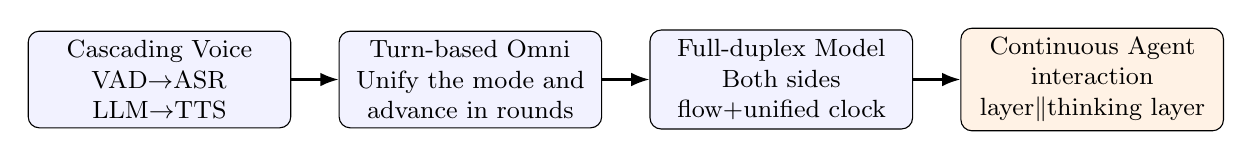
\begin{tikzpicture}[node distance=6mm,>=Latex,font=\small,
box/.style={draw,rounded corners,minimum height=10mm,text width=31mm,align=center,fill=blue!5},
arr/.style={->,thick}]
\node[box] (c1) {Cascading Voice\\VAD$\to$ASR\\LLM$\to$TTS};
\node[box,right=of c1] (c2) {Turn-based Omni\\Unify the mode and advance in rounds};
\node[box,right=of c2] (c3) {Full-duplex Model\\Both sides flow+unified clock};
\node[box,right=of c3,fill=orange!10] (c4) {Continuous Agent\\interaction layer$\parallel$thinking layer};
\draw[arr] (c1)--(c2);
\draw[arr] (c2)--(c3);
\draw[arr] (c3)--(c4);
\end{tikzpicture}
\caption{The key evolution of speech models is not to simply expand parameters, but to gradually remove text bottlenecks, turn barriers and single-time scale reasoning.}
\label{en:fig:evolution}
\end{figure}

\subsection{Official system profile of GPT-Live}

The online system described by \FOne OpenAI can be summarized into four planes. First, the \textbf{ media plane (media plane) } continuously sends and receives audio through WebRTC, and handles packet loss, jitter, clock drift and audio catch-up. Second, the \textbf{ interaction plane } runs the GPT-Live speech model and continuously decides when to speak, listen, stop, interrupt, call tools, or initiate delegation according to the audio clock. Third, \textbf{ cognitive plane } maintains a pre-created and populated frontier-model session with stable session affinity for undertaking complex reasoning. Fourth, \textbf{ control/state plane } maintains session state, transcript, context compaction, security control and instance handoff \cite{en:openai2026continuous,en:openai2026safety}.

Set up an asynchronous RPC\footnote{Remote Procedure Call between the media fast path and the application logic. } Boundaries are critical: neither database access, business logic, nor time-consuming tools can reversely block audio frames. The system therefore has two consistency levels: the audio path adopts a "time-limited priority" weak synchronization method, and the application state adopts retryable event semantics. Discrete semantic turns can still be derived on top of continuous audio, and both speculative transcript and authoritative transcript are maintained simultaneously. Therefore, "cancelling the turn detector" refers to canceling the turn gating that would block the audio path, rather than giving up semantic segmentation.

\begin{figure}[H]
\centering
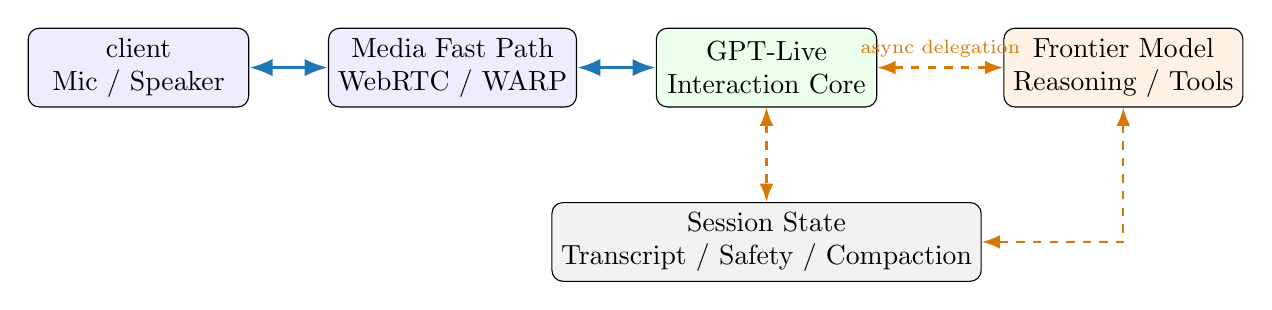
\begin{tikzpicture}[>=Latex,node distance=8mm and 10mm,
p/.style={draw,rounded corners,minimum width=28mm,minimum height=10mm,align=center},
fast/.style={->,very thick,official},slow/.style={->,thick,dashed,hypothesis}]
\node[p,fill=blue!7] (client) {client\\Mic / Speaker};
\node[p,fill=blue!7,right=of client] (media) {Media Fast Path\\WebRTC / WARP};
\node[p,fill=green!8,right=of media] (live) {GPT-Live\\Interaction Core};
\node[p,fill=orange!10,right=16mm of live] (think) {Frontier Model\\Reasoning / Tools};
\node[p,fill=gray!10,below=12mm of live] (state) {Session State\\Transcript / Safety / Compaction};
\draw[fast,<->] (client)--(media);
\draw[fast,<->] (media)--(live);
\draw[slow,<->] (live)--node[above,font=\scriptsize]{async delegation}(think);
\draw[slow,<->] (live)--(state);
\draw[slow,<->] (think)|-(state);
\end{tikzpicture}
\caption{Outlines of the GPT-Live system under evidence constraints. The solid blue line is the low-latency media closed loop, and the orange dashed line is the cognitive and state closed loop that allows higher latency. The logical layering in the figure comes from official facts; the internal implementation of the module remains undisclosed.}
\label{en:fig:official-architecture}
\end{figure}

\section{Formalizing Full-Duplex Continuous Inference}

The round-robin LLM only needs to ensure the causality on the token sequence; the full-duplex model must also ensure that the queuing and calculation time of each audio chunk meets $Q_t+C_t\leq\Delta$. Otherwise, even if the semantics are correct, lags will occur due to missing the playout deadline. Therefore, the state of continuous inference not only contains historical semantics, but also must synchronize user audio, assistant's own output, playback progress, tool events, and safety signals, and allow low-latency interaction paths and high-cost cognition paths to advance in parallel on different time scales.

\subsection{From token sequence to wall-clock constrained two-stream process}

The following formalization uses standard Transformer autoregressive modeling as a starting point \cite{en:vaswani2017attention}.

Ordinary autoregressive LLM modeling $p(y_n\mid x,y_{<n})$, input $x$ is fixed before decoding starts. Full-duplex speech is different: new user input continues to arrive while the assistant generates speech. Discretize the wall-clock into audio chunks of length $\Delta$, let $u_t$ represent the $t$ user audio chunk, $a_t$ represent the assistant output, $z_t$ represent the internal interaction action, and $m_t$ represent the persistent state, then the system needs to complete the following calculations before each playout deadline:
\begin{align}
m_t &= f_\theta(m_{t-1},u_t,\tilde a_{t-d:t-1},e_t),\\
(a_t,z_t) &\sim p_\theta(\cdot\mid m_t),\qquad
z_t\in\{\texttt{listen,speak,pause,stop,backchannel,delegate,tool}\}.
\end{align}
$\tilde a$ represents the system's own playback reference, or its own output after acoustic echo cancellation; $e_t$ represents tool results, network status, and safety signals. The most important constraint here is not the probability formula itself, but $C_t+Q_t\leq\Delta$: the sum of the calculation time $C_t$ of a single audio chunk and the queuing time $Q_t$ must be less than the playout deadline. Occasional timeouts will cause audio underrun, and continuous timeouts will appear as mechanical pauses.

Full-duplex contains at least four meanings: (1) The transport layer can be uplinked and downlinked at the same time; (2) The model continues to encode user input while speaking; (3) The policy layer can handle speech overlap, short responses and user interruptions; (4) The session layer remains interactive during the execution of background tasks. Merely having a two-way WebSocket connection cannot be called a full-duplex model; if the system freezes interaction when processing complex tasks, even if it has the first three layers of capabilities, it is not equivalent to the continuous agent emphasized by GPT-Live.

\subsection{State, Causality, and Echo}

The causal system can only use $u_{\le t}$, but in exchange for a more robust speech representation, has limited look-ahead $L$. The algorithm delay lower bound is approximately
\begin{equation}
T_{\mathrm{algo}}=T_{\mathrm{chunk}}+T_{\mathrm{lookahead}}+T_{\mathrm{codec}}+T_{\mathrm{decode}}.
\end{equation}
Reducing $\Delta$ will increase decision frequency, but increase token rate, kernel launch and scheduling pressure. Publicly available systems with a time grid of 80--160 ms represent a typical compromise: fast enough to respond to interruptions, yet able to accumulate discernible acoustic evidence within a grid \cite{en:defossez2024moshi,en:zhang2026duplexsla}.

The model must also differentiate between "the user is speaking" and "the speaker sound is being reacquired by the microphone." Traditional AEC\footnote{Acoustic Echo Cancellation, acoustic echo cancellation. } eliminates known playback references in the waveform domain; the model side can also explicitly receive assistant history, self-output token or echo flag. If only a single channel of mixed audio is used for training, the model may mistake its own voice for user instructions. SALMONN-omni lists echo cancellation as the full-duplex core scenario \cite{en:yu2025salmonnomni}, indicating that the evaluation must cover residual echo, double talk and different acoustic paths, and cannot only be tested on clean separate channels.

\subsection{Dual time scale control}

Control latencies for natural conversation are not the same as task reasoning latencies. The fast ring $\pi_f$ runs every $\Delta$ milliseconds and is responsible for maintaining contact and deciding whether to give up the floor; the slow ring $\pi_s$ may run for several seconds and is responsible for searching, planning, or calling tools:
\begin{equation}
\pi_f:(u_t,m_{t-1})\mapsto(a_t,z_t),\qquad
\pi_s:(q,M)\mapsto r,quad r\xrightarrow{\mathrm{event}}m_{t+k}.
\end{equation}
The difficulty with asynchronous delegation is how to re-inject the results into the current conversation: the results may be out of date, the task may be canceled by the user, or they may conflict with previous representations of the interaction layer. Therefore, the event should at least contain \texttt{task\_id}, context version, creation time, cancellation status and source information; after receiving the result, the interaction layer should also perform a correlation judgment instead of unconditional reading.

\section{Public Model Architectures: Components and Design Axes}

Although the public models in recent years have different implementation paths, they have gradually converged to the basic structure of "shared timeline, dual streams of users and assistants, and continuous status updates". What really affects the behavior of the system are three sets of tradeoffs: the uniformity of generation and high token rate of codec tokens, the semantic coupling capability and overlap interference of channel fusion, and the control accuracy and backbone burden of silence/control/action tokens. These design axes can explain the differences between Moshi, SyncLLM, LSLM, Neural-FSM and DuplexSLA, and also constitute a candidate mechanism space for understanding GPT-Live.

\subsection{Audio representation: continuous features, semantic tokens and codec tokens}

End-to-end voice LLM typically starts by downsampling the 16/24 kHz waveform to a low-frequency representation. SoundStream and EnCodec use a convolutional encoder, residual vector quantization (RVQ), and a generative decoder to compress the waveform into a multi-codebook discrete token\cite{en:zeghidour2021soundstream,en:defossez2022encodec}. If the frame rate is $f$, the number of codebooks is $K$, and the size of each dictionary is $V_k$, the original discrete code rate
\begin{equation}
R=f\sum_{k=1}^{K}\log_2V_k\quad\text{bit/s}.
\end{equation}
High-level codebooks tend to carry coarser semantics and prosody, with subsequent codebooks filling in the acoustic details. AudioLM further separates semantic tokens and acoustic tokens, uses lower-frequency semantics to ensure long-term consistency, and uses codec code to reconstruct the sound quality \cite{en:borsos2022audiolm}.

VITA-Audio uses multiple cross-modal token prediction to generate multiple audio tokens in one forward pass. The author reports that 3--5 times the inference speedup\cite{en:long2025vitaaudio} is obtained at the 7B scale, indicating that parallel acoustic decoding is an important direction to reduce time-to-first-audio.

The Codec-token route allows next-token prediction to cover both understanding and generation, but the token rate is very high. Assume 12.5 frames per second and 8 codebooks, that is, 100 audio tokens per second; if both streams exist at the same time, backbone throughput and KV cache\footnote{Key-Value cache, Transformer caches the Key and Value representation of historical tokens during incremental decoding to avoid repeated calculations. } growth will be significantly higher than text chat. Typical optimizations include delay pattern, hierarchical depth decoder, multi-token prediction, and semantic/acoustic layering. Moshi uses Temporal Transformer to model time, Depth Transformer to expand multiple codebooks in the same frame, and time-aligned text Inner Monologue to improve language quality \cite{en:defossez2024moshi}.

Another route does not inject the codec id into the LLM vocabulary. LSLM uses streaming SSL\footnote{Self-Supervised Learning, self-supervised learning; here it refers to learning continuous acoustic representations with unlabeled speech. } encoder provides continuous auditory features and token-based TTS to generate speech; SALMONN-omni emphasizes codec-free token space and dynamic thinking \cite{en:ma2025lslm,en:yu2025salmonnomni}. This approach reduces the acoustic entropy that the backbone needs to learn, but requires an external speech decoder to strike a balance between low latency and high fidelity. The two types of routes are essentially the difference in the division of labor on "how much acoustic details the backbone bears."

A recent review summarized related methods as "engineering synchronization" and "learning synchronization", which also confirmed that the model side and the system side need to evolve in parallel \cite{en:chen2025survey}.

\subsection{Representing Both Speakers in the Backbone}

\paragraph{Sequence flattening}
SyncLLM cuts real time into chunks and serializes user and assistant events with synchronization markers; OmniFlatten uses a unified flatten operation to cover modal alignment, half-duplex and full-duplex training \cite{en:veluri2024syncllm,en:zhang2024omniflatten}. The advantage is that it reuses standard decoder-only LLM and next-token loss. The disadvantage is that the sequence order may artificially break the symmetry of "the same moment" and the token rate will be inflated.

\paragraph{Parallel streams and multiple codebooks}
Moshi simultaneously models user and assistant audio streams, and dGSLM earlier used Twin Towers Transformer and cross-attention to generate speech, laughter and turn dynamics \cite{en:nguyen2022dgslm,en:defossez2024moshi} in two channels in parallel. Parallel representation is closest to the physical process, but batch, cache and loss mask all need to understand the two-dimensional time $\times$ channel structure.

\paragraph{Fusion and cross-attention}
LSLM compared early, middle and late fusion. A control experiment in 2026 further showed that channel fusion can establish stronger semantic connections, but it is also easier to interfere with the generated context when input overlap; using user stream as external memory and reading through cross-attention is more robust, but the question and answer ability is relatively weak \cite{en:ma2025lslm,en:lu2026routing}. Therefore, architecture evaluation cannot only look at static spoken QA, but must also examine semantic recovery after interruption.

\subsection{Representing Interaction Actions}

The simplest approach is to treat silence as an output: if the model generates a silence token at a certain time slot, it means that it has chosen to "continue listening". SyncLLM and Moshi can implicitly learn overlaps and pauses from the joint distribution of the user and assistant streams. Neural-FSM allows LLM to explicitly output the control token and drive a dual-state FSM\footnote{Finite-State Machine, a finite state machine. }, decide to start answering, continue waiting, or accept interruption; the paper reports that in simulation evaluation, its average response delay was more than three times lower than that of the half-duplex system, and more than half of the interactions could respond to \cite{en:wang2024neuralfsm} within 500 ms. Explicit control makes monitoring and auditing easier, but a state machine that is too coarse-grained can also limit the naturalness of interactions.

DuplexSLA combines decoding assistant audio with a rate-limited text action channel on a shared 160 ms timeline, allowing planning and tool invocation to occur in parallel with speech output\cite{en:zhang2026duplexsla}. This represents a more general speech--language--Action (Speech--Language--Action, SLA) modeling method: audio is responsible for low-bandwidth social feedback, and the action channel is responsible for high-precision structured control. GPT-Live officially only confirms that the system can continuously decide when to call tools or initiate asynchronous delegation; whether there are native action headers internally has not yet been disclosed.

\begin{table}[H]
\centering\scriptsize
\setlength{\tabcolsep}{3pt}
\caption{The core design axis of the full duplex public route. "GPT-Live" in the table only lists official public attributes, and the question mark indicates that it has not been disclosed.}
\begin{tabularx}{\textwidth}{lXXXXX}
\toprule
System & Input organization & Voice output & Interactive control & Deep reasoning & Main features \\
\midrule
Moshi & Dual parallel audio streams & RVQ codec & Implicit timing & Single trunk & Inner Monologue, about 200 ms Actual measurement \\
SyncLLM & time chunk flattening & HuBERT/voice unit & sync token & single trunk & real clock synchronization \\
Neural-FSM & serialized sensing event & modular motor & control token & within LLM & two-state FSM \\
LSLM & streaming SSL & token TTS & post-fusion prediction & single-backbone & early/middle/late fusion \\
OmniFlatten & flatten sequence & speech token & learning from data & single-backbone & three-stage post-training \\
SALMONN-omni & Continuous speech features & Independent generation module & dynamic thinking & Single backbone & codec-free token space \\
DuplexOmni & streaming audio/video & streaming voice & interaction layer & asynchronous plug-in & interaction -- thinking decoupling \\
DuplexSLA & Dual-stream three-channel & Discrete audio & action channel & Same as trunk action & Shared 160 ms clock \\
GPT-Live & Continuous audio & Continuous voice & Continuous decision-making & Asynchronous delegation & tokenizer/fusion Undisclosed \\
\bottomrule
\end{tabularx}
\end{table}

\subsection{The essential difference from the end-to-end Omni Model}

The two are not mutually exclusive concepts. Omni emphasizes \emph{ modal unity }: the same model can understand and generate text, images or audio; full-duplex emphasizes \emph{ time and control unity }: new inputs can continue to arrive during the generation process, and the model can sense wall-clock, and maintain the correct causal state when speech overlaps. A model can be Omni but still interact on a turn-by-turn basis, or it can be full-duplex capable but only handle audio.

GPT-Live further introduces \emph{ capability decoupling }: the low-latency interactive core does not have to bear all complex reasoning. Rather than having the very large omni model complete an expensive inference every 80--160 ms, this solution allocates "frame-level decisions that cannot be missed" and "tasks that can wait but require smartness" to different computing paths. This is both product experience design and the core of serving feasibility.

\section{Training data and post-training}

\subsection{Why Is Ordinary Voice Q\&A Data Insufficient?}

Turn-based SFT\footnote{Supervised Fine-Tuning, supervised fine-tuning. } samples usually only have "complete user audio $\to$ complete assistant answer", with almost no overlap, hesitation, short feedback, talk grabbing, cancellation and self-correction. The model is ASR, SQA\footnote{Spoken Question Answering, spoken question answering. } and TTS are both very strong, and they will only wait for the end of the clear sentence. Full-duplex training samples should be binaural, shared timeline event sequences
\begin{equation}
D=\{(u_{1:T},a_{1:T},c_{1:T},s_{1:T},q,r)\},
\end{equation}
Among them, $c_t$ is the interaction action, $s_t$ is the speaker/overlapping state, and $q,r$ is the optional delegation request and return. Data must not only answer "what to say" but also monitor "when to speak, when to remain silent, and when to stop."

Real binaural data are scarce and privacy sensitive. SyncLLM trained the clock synchronization capability \cite{en:veluri2024syncllm} with 212k hours of synthetic speech dialogue and 2k hours of real dialogue; DuplexChat-Pipe performed language filtering, download cleaning, diarization, dual-person segment extraction, speech separation and restoration from public podcasts, and the author reported output of 282,634 hours of English and 132,723 hours of Japanese data \cite{en:nakata2026duplexchat}. These scales mean that data engineering has become a major constraint on model capabilities, but automatic separation introduces crosstalk, mis-speakers, false overlaps and recovery artifacts, and quality tags must be preserved rather than just reported in hours.

\subsection{Suggested Progressive Training Recipes}

Progressive training is commonly used in public work. OmniFlatten sequentially performs modal alignment, half-duplex dialogue learning, and full-duplex dialogue learning \cite{en:zhang2024omniflatten}; Freeze-Omni freezes the text backbone, first accesses the voice input and output modal, and then performs duplex multi-task training \cite{en:wang2024freezeomni}. A reproducible six-stage training program is as follows:

\begin{enumerate}
\item \textbf{Representation pretraining: } optimizes reconstruction quality, semantic fidelity, streaming causality and low frame rate to establish a stable representation under clean/noisy/echo conditions.
\item \textbf{Speech--text alignment: } mixes ASR, TTS, speech continuation, and spoken QA to align speech capabilities with the text backbone; replay text capabilities to avoid catastrophic forgetting.
\item \textbf{Half-duplex dialogue: } Learn command following, roles, voice style and long context to ensure "what to say" converges first.
\item \textbf{Synthetic duplex conversion: } expands text conversations into timestamped binaural audio, randomly sampling pauses, backchannels, overlaps, barge-in and network delays.
\item \textbf{Real duplex adaptation: } uses real two-channel dialogue to calibrate time distribution, prosody and cultural differences, reducing template bias in synthetic data.
\item \textbf{Preference/RL\footnote{Reinforcement Learning, reinforcement learning. }: } optimizes interruption accuracy, error grabbing, task completion, conversation redundancy and recovery capabilities; introduces safety interrupt and delegate policy.
\end{enumerate}

The loss can be written as
\begin{equation}
\mathcal L=\lambda_a\mathcal L_{audio}+\lambda_t\mathcal L_{text}+\lambda_c\mathcal L_{control}
+\lambda_{asr}\mathcal L_{align}+\lambda_s\mathcal L_{safety}+\lambda_d\mathcal L_{delegate}.
\end{equation}
The magnitudes of tokens corresponding to different losses vary greatly. The density of audio tokens is much higher than that of control tokens; if simply averaged by token, the model will prioritize optimizing acoustic details and ignore rare but critical correct interruptions. Therefore, control/action events should be reweighted, and precision/recall should be reported by scenario instead of just looking at the total loss.

\subsection{Quantifiable quality control of data pipelines}

It is recommended that the following quality fields be retained for each audio segment: Speaker Purity, Overlap Ratio, Signal-to-Noise Ratio, Residual Echo, Speaker Separation Confidence, Speech Separation Artifact Score, Language and Accent, Turn Switch Interval, Short Answer Label, Privacy and Security Label, and Licensed Source. Key thresholds include: (1) Crosstalk leakage is determined when binaural cross-correlation is too high; (2) Sample weights are reduced when ASR transcription is inconsistent with the speaker's timeline; (3) Extreme negative intervals and long overlaps are bucketed separately; (4) Between the training set and the evaluation set, the same podcast, the same speaker, and near-duplicate audio are deduplicated.

For synthetic data, \emph{ two-way calibration } is required: first, the target distribution of the round switching interval, overlap duration and short response frequency is given by the real data, and the synthesizer then samples according to these distributions; after the training is completed, it is also necessary to check whether the model output deviates from the true distribution. Simply pursuing lower response latency will induce the model to frequently grab calls, so the false interruption rate must also be used as a protection indicator.

\section{Stateful Serving: Delivering Audio Frames on Time}

The upper limit of the capacity of real-time voice serving is not how many requests are completed per unit time, but how many concurrent sessions can continue to generate audio frames before their respective playout deadlines; the average RTF\footnote{Real-Time Factor, real-time factor; usually refers to the ratio of the time required to process a piece of audio to the length of the audio piece. } less than 1 may still cover up consecutive deadline misses caused by burst prefill. Long sessions will also cause the KV cache to continue to grow with audio tokens, so context compaction must be moved out of the live path, and smooth handoff must be completed through background prefill, parallel running, and safe cut-over of the replacement instance.

\subsection{From Request Capacity to Session-Frame Capacity}

Text serving can use single request latency instead of throughput; real-time voice cannot make the session wait for long prefill.

\FOne OpenAI clearly measures capacity by "how many concurrent sessions can continue to process frames on time" instead of GPU request throughput\cite{en:openai2026continuous}.

Assuming that the active session set is $S$ and the $i$ session frame budget is $\Delta_i$, the more reasonable SLO\footnote{Service-Level Objective is the service level objective. } Yes
\begin{align}
\mathrm{DMR} &= \frac{\sum_{i,t}\mathbf 1[Q_{i,t}+C_{i,t}>\Delta_i]}{\sum_iT_i},\\
\mathrm{GoodSessions} &= \sum_i\mathbf 1[\mathrm{DMR}_i<\epsilon\land P_{99}(J_i)<J_{max}],
\end{align}
Here we measure the deadline-miss ratio (DMR) \footnote{Deadline-Miss Ratio respectively, which is the proportion of frames that failed to complete before the deadline. } and the number of concurrent sessions that meet the jitter threshold. Even if the average real-time factor (RTF) is lower than 1, the interactive experience is not guaranteed because sudden context prefill may still cause continuous frame misses.

The scheduler should use deadline-aware continuous batching: sort audio frames according to the latest playout deadline; limit the size of each batch of context prefill; reserve computing power for audio decode; put background context compaction, transliteration revision, and delegation model prefill into a low-priority queue. When the load is too high, you should successively reduce non-critical telemetry, reduce the intensity of acoustic refinement, delay background tasks, and finally consider sacrificing the quality of the interactive core.

\subsection{KV cache and continuous context}

Transformer-XL's segment recurrence is an earlier cross-segment memory solution \cite{en:dai2019transformerxl}, but real-time voice also requires that the state and playback time are strictly consistent.

The Transformer KV cache grows over time at every layer. Its GPU-memory footprint is approximately
\begin{equation}
M_{KV}\approx 2LNH_{kv}d_hb,
\end{equation}
Among them, $L$ is the number of layers, $N$ is the cumulative token, $H_{kv}$ is the number of KV heads, $d_h$ is the head dimension, and $b$ is the bytes per element. The combination of high audio token rate and long sessions makes the cache become the session capacity bottleneck. PagedAttention reduces dynamic cache fragmentation and duplication through paging, and FlashAttention reduces attention to HBM access \cite{en:kwon2023pagedattention,en:dao2022flashattention} through IO-aware tiling; but they do not automatically resolve infinite contexts.

Hierarchical memory can be used: (1) retain the original dual-stream token for the most recent $W$ seconds to ensure interruption processing and reference resolution; (2) compress earlier speech into final transcription and event summary; (3) retain structured provenance for tool results; (4) write user preferences into independent long-term states. Compression is not a lossless operation, it changes the token prefix and invalidates the old KV cache. \FOne OpenAI moves the context compaction out of the live path, completes the prefill of the replacement instance in the background, and then switches to \cite{en:openai2026continuous}, thereby preventing the main instance from stalling due to long context prefill.

\subsection{Seamless instance switching}

Stateful sessions cannot be arbitrarily load balanced like normal HTTP requests. The officially described switching process is: start and warm up replacement; prefill with compressed context; run new and old instances in parallel; cut over at safety boundaries. This process simultaneously addresses context compression, instance maintenance, and failure recovery.

\begin{figure}[H]
\centering
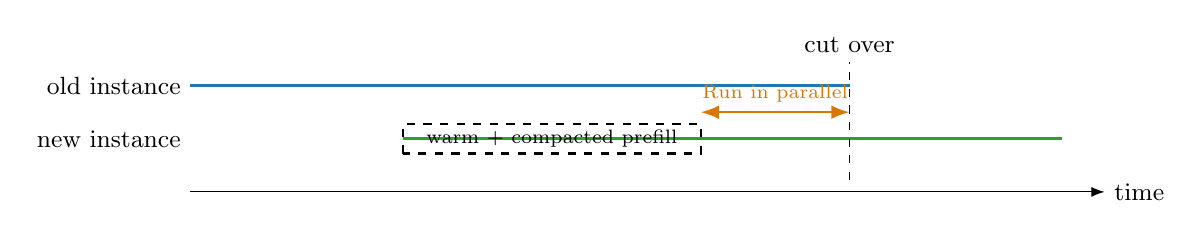
\begin{tikzpicture}[>=Latex,x=1.35cm,y=0.75cm,font=\small]
\draw[->] (0,0)--(8.6,0) node[right]{time};
\node[left] at (0,1.8){old instance}; \node[left] at (0,0.9){new instance};
\draw[very thick,official] (0,1.8)--(6.2,1.8);
\draw[very thick,public] (2.0,0.9)--(8.2,0.9);
\draw[thick,dashed] (2.0,0.65) rectangle (4.8,1.15);
\node[font=\scriptsize] at (3.4,0.9){warm + compacted prefill};
\draw[<->,hypothesis,thick] (4.8,1.35)--(6.2,1.35) node[midway,above,font=\scriptsize]{Run in parallel};
\draw[dashed] (6.2,0.2)--(6.2,2.2) node[above]{cut over};
\end{tikzpicture}
\caption{Stateful reasoning instance switching. Switching points should be at recoverable acoustic boundaries, and duplicate/missing frames should be deduplicated.}
\end{figure}

There are three types of race conditions that need to be dealt with in the project: the tool results arrive exactly during the instance switch; the final transcriber revise the old text; and the user interrupts at the flow boundary. It is recommended to attach a monotonically increasing sequence number and context epoch to all events; the new instance only accepts state changes matching the epoch, and deduplicates the media frame according to the playout timestamp.

\subsection{Asynchronously delegated serving design}

\FOne In order to reduce the first response delay of complex tasks, the system will pre-create and populate the frontier-model session, maintain stable session affinity, and utilize prompt caching\cite{en:openai2026continuous}. The time taken for delegation can be broken down into
\begin{equation}
T_{delegate}=T_{route}+T_{queue}+T_{prefill\_delta}+T_{reason}+T_{tool}+T_{return}.
\end{equation}
Pre-population can only reduce $T_{prefill\_delta}$; inference strength, the size of the tool pattern definition, and the number of serial tool call rounds still determine long-tail latency. Therefore, the interaction layer needs to adopt progressive feedback: first use a short response to inform the user that the task is being processed, and then choose the appropriate time to insert after the result arrives; if the user has changed the topic, cancel the background task or reduce its priority.

Speculative decoding can first generate a draft from a small model and then hand it over to a large model for parallel verification, reducing the serial decoding step\cite{en:leviathan2023speculative} without changing the target distribution; however, it is more suitable for the cognition path and cannot replace the scheduling with hard deadline constraints in the interaction path.

Security policies must also be consistent across layers. The GPT-Live system card claims that the security system continuously checks input and output along with the conversation and can steer, interrupt, play a security response or end the session \cite{en:openai2026safety}. This means that security controls cannot just sit at the end of the delegated model, otherwise the real-time layer may have generated inappropriate speech before the long inference returns.

\section{Real-time networking: WebRTC, WARP and playout clock}

\subsection{Why not "just switch to WebSocket"}

WebRTC converts media, NAT\footnote{Network Address Translation, network address translation; NAT traversal refers to establishing an end-to-end connection across address translation devices. } penetration, congestion control, security and data channels are combined into a browser real-time communication stack. In standard WebRTC, media usually passes through the SRTP\footnote{Secure Real-time Transport Protocol. }, non-media data channel uses SCTP over DTLS over ICE/UDP \footnote{SCTP: Stream Control Transmission Protocol, flow control transmission protocol; DTLS: Datagram Transport Layer Security, datagram transport layer security protocol; ICE: Interactive Connectivity Establishment, interactive connection establishment; UDP: User Datagram Protocol, user datagram protocol. }\cite{en:alvestrand2021webrtc,en:jesup2021datachannels}. Audio frames have different reliability requirements than tool events: old audio packets that arrive late are usually not worth retransmitting, while tool results and status changes need to be reliable and orderly. Putting both into a reliable byte stream creates head-of-line blocking.

The end-to-end perceived delay can be written as
\begin{equation}
T_{e2e}=T_{capture}+T_{uplink}+T_{jitter,in}+T_{model}+T_{downlink}+T_{jitter,out}+T_{playout}.
\end{equation}
If the 20 ms saved on the model side is offset by the 300 ms connection setup or jitter buffer, the user will not perceive this part of the optimization. On the contrary, if the jitter buffer is too small, it will increase the number of missing frames in a weak network environment. The system should be based on recent packet loss, RTT\footnote{Round-Trip Time, and round-trip delay, which is the time required for data to travel from the sender to the receiver and back again. } and clock drift dynamically adjust the playout policy instead of setting the same fixed parameters for the global network.

SimulTron's end-side synchronous speech-to-speech translation is also jointly designed with the causal encoder, adjustable fixed delay and streaming vocoder \cite{en:agranovich2024simultron}, indicating that both the model algorithm and the audio playback path must be taken into account when evaluating delay.

\subsection{Optimization of connection establishment from 6 RTT to 1 RTT}

\FOne OpenAI collectively refers to related WebRTC optimizations as WARP, saying that the establishment of media and data channels is reduced from 6 round trips to 1, combined with SPED\footnote{STUN Protocol for Embedding DTLS; where STUN is Session Traversal Utilities for NAT. This draft embeds DTLS handshake data and acknowledgment into STUN Binding messages. }, DTLS 1.3, SNAP\footnote{SCTP Negotiation Acceleration Protocol, put SCTP initialization parameters into SDP offer/answer to reduce serial round-trips for data channel establishment. } and pre-negotiated data channel\cite{en:openai2026continuous}. DTLS 1.3 itself uses the shorter handshake mode \cite{en:rescorla2022dtls13}; SPED embeds DTLS handshake data/ack into STUN Binding Request/Response; SNAP embeds SCTP initialization parameters into SDP\footnote{Session Description Protocol. } offer/answer, thereby reducing the serial round trip of the data channel \cite{en:hancke2026sped,en:hancke2026snap}. The latter two are still Internet-Draft as of this writing and cannot be considered stable RFC\footnote{Request for Comments, a series of standards, specifications, or informational documents in the field of Internet engineering and protocols. }.

Instant Connect goes one step further and pre-negotiates SDP, allowing the client to start session \cite{en:openai2026continuous} with a single UDP packet. This requires the server to allocate or restore sufficient connection status in advance, and also introduces anti-replay, resource abuse, and reservation expiration issues. Low RTT is not a free lunch: the more aggressive the state warm-up, the higher the cost due to air connections and attack traffic.

\subsection{Packet Loss, Clock Drift, and Audio Catch-Up}

The client sampling clock, server generation clock and speaker playout clock are not completely consistent. If the generation is slightly slower, the buffer will gradually be exhausted; if the generation is slightly faster, the buffer accumulation will cause the interaction to become later and later. The official article mentions audio time stretching/catch-up\cite{en:openai2026continuous}: Adjust the playout rate within a small range or selectively discard low-value segments to bring the delay back to the target range. Implementations should limit the stretching ratio and operate at the voice activity boundary to avoid pitch and prosody distortion.

The weak network test at least covers independent random packet loss and burst loss, uplink/downlink asymmetry, RTT burst, NAT rebinding, Wi-Fi/cellular switching, client background recovery and audio device switching. The evaluation is not only the ASR after packet loss WER\footnote{Word Error Rate, the word error rate is usually calculated based on the number of substitution, deletion and insertion errors relative to the reference word count. }, also includes whether the assistant repeats, grabs the call, forgets the user's mid-course correction, and whether the tool events are consistent with the audio status.

\section{Evaluation: From Model Scores to Continuous Interaction Quality}

\subsection{Four-tier evaluation framework}

Full-Duplex-Bench splits the core interaction behaviors into pause processing, short responses, turn switching and interruption management \cite{en:lin2025fullduplexbench}; v2 further adds multi-round stage goals, fast and slow speaking rhythms, error correction, entity tracking and security tasks \cite{en:lin2026fullduplexbenchv2}. Combined with the online system requirements, it is recommended to conduct evaluation from the following four levels:

\begin{enumerate}
\item \textbf{ Acoustics/Semantics: }ASR WER, spoken QA accuracy, speaker similarity, MOS\footnote{Mean Opinion Score, average subjective opinion score, usually evaluated by the listener for naturalness or quality of speech; UTMOS is automatically predicted MOS Neural network evaluator. }/UTMOS, mood and prosody following, noise/accent robustness.
\item \textbf{ Interaction behavior: } initial response delay, pause/overlap distribution, accuracy and recall rate of short responses, stop delay after user interrupts, false interruption rate, and semantic consistency after recovery.
\item \textbf{ agent tasks: } tool calling accuracy rate, parameter exact matching rate, delegation trigger accuracy and recall rate, task completion rate, cancellation instruction compliance rate, result timeliness and source information accuracy rate.
\item \textbf{ System service quality: }connection RTT, first audio delay, audio frame deadline-miss ratio, jitter, playout buffer underrun, handoff gap, single session GPU memory, number of sessions each GPU can stably carry, and cost per minute.
\end{enumerate}

There are cultural differences in human turn-taking itself\cite{en:stivers2009turntaking}, therefore the single "faster, better" cannot be regarded as a natural goal. The full distribution of transition gaps should be reported, and the reviewer should be asked to simultaneously rate response relevance, abruptness, verbosity, and respect for interruptions.

\subsection{Key Metric Definitions}

Assume that the user starts interrupting at time $t_b$ and the assistant stops audible speech at time $t_s$, then the stop delay is $t_s-t_b$; only when the user input does constitute a valid semantic interruption, it will be recorded as a real example. defined by this
\begin{equation}
P_{int}=\frac{N_{correct\ stop}}{N_{all\ stop}},\qquad
R_{int}=\frac{N_{correct\ stop}}{N_{valid\ barge\mbox{-}in}}.
\end{equation}
Optimizing only $R_{int}$ may cause the model to stop speaking due to coughing or short responses; optimizing only $P_{int}$ may cause the model to appear to be "rushing to talk" all the time. Therefore, $F_1$, cessation latency quantile, and recovery success rate should be reported simultaneously.

Delegation should be evaluated counterfactual: compare no delegation, synchronous delegation, and asynchronous delegation for the same task. Metrics include interaction stall, final accuracy, first useful feedback, tool round trips, and wasted computing power after user cancellation. The value of an asynchronous approach is not to make the final answer necessarily faster, but to keep the conversation available during slow tasks.

\subsection{Experiment Matrix and Attribution Principles}

To avoid confounding factors, it is recommended to fix the backbone, training token, duplex/real data ratio, codec, hardware and network trace, and only change one design axis. FIFO\footnote{First In, First Out in the table. } and EDF\footnote{Earliest Deadline First, the earliest deadline takes precedence. } is a two-type scheduling baseline, and the core ablation is as follows:

\begin{table}[H]
\centering\small
\caption{Proposed attributable ablation experiments.}
\begin{tabularx}{\textwidth}{p{3.0cm}p{4.0cm}X}
\toprule
Design axis & Control group & Main indicators and expected risks \\
\midrule
User flow routing & Channel fusion / cross-attention / gated mixing & SQA, post-overlap semantic interference, stop delay \\
Time granularity & 40/80/160/320 ms & DMR, interrupt delay, token throughput, voice naturalness \\
Action expression & Only silence token / FSM control token / action channel & Control accuracy, precise matching of tool parameters, backbone burden \\
Training plan & Direct full-duplex / three-stage / six-stage & Convergence, text ability forgetting, real interaction scoring \\
Thoughts on interaction -- & Single model / synchronous delegation / asynchronous delegation & Interaction pause, task accuracy, cost, cancellation waste \\
Context management & sliding window / summary / background handoff & long-session consistency, handoff gap, KV-cache GPU memory \\
Scheduling strategy & FIFO / continuous batching / EDF + computing power reservation & Stable number of sessions per GPU, DMR, P99 jitter \\
Network & Standard WebRTC / 1-RTT optimization / pre-connected & connect latency, security and air connection cost \\
\bottomrule
\end{tabularx}
\end{table}

Each result reports at least the mean, and P50/P95/P99\footnote{ represent the 50th, 95th, and 99th percentiles respectively; P99 is often used to observe the long-tail delay of the system. }, confidence interval and sample size by scenario. The randomness of the speech model and network traces will amplify the variance; if only one demo or average latency is reported, architectural conclusions cannot be supported.

\section{GPT-Live architecture reconstruction under evidence constraints}

Public evidence can confirm that GPT-Live continuously listens when making sounds, makes interaction decisions based on fine-grained clocks, and asynchronously delegates complex tasks to the frontier model; but these facts are not enough to deduce its specific tokenizer, fusion location, or action head. The minimal reconstruction that satisfies these constraints is a hybrid architecture: the media fast path carries continuous audio, the stateful interaction core maintains the two-stream causal state, the action channel triggers tools and delegation, the asynchronous cognition plane handles slow inference, and the authoritative state handles transcription, security, and context compaction.

\subsection{Which parts can be determined}

Based on official materials, the following system properties can be determined: \FOne (1) The speech model continues to listen when speaking, and does not use the traditional turn detector as a driving condition for audio processing; (2) The model decides multiple times per second when to speak, listen, pause, accept interruptions, call tools, or initiate delegation; (3) Complex tasks can be delegated asynchronously while maintaining uninterrupted interaction; (4) The media fast path and application logic are controlled by asynchronous RPC. Isolation; (5) Session inference has persistent state and supports background pre-population and instance switching; (6) Context compression does not block the real-time path; (7) WebRTC/WARP, packet loss processing and clock drift correction jointly determine the end-to-end experience; (8) System capacity is measured by whether the session audio frame can be completed on time \cite{en:openai2026gptlive,en:openai2026continuous}.

Together, these properties rule out two oversimplified explanations. First, GPT-Live is unlikely to be just "faster ASR, LLM, and TTS" because such pipelines rely on discrete rounds and cannot naturally handle new inputs arriving during the system's voicing. Second, it should not be understood as "one very large model taking on all tasks", because the official statement clearly states that the system will asynchronously hand over complex tasks to the cutting-edge model for processing.

\subsection{The most credible but unconfirmed internal mechanism}

The \Hyp interaction core is likely to have an internal state equivalent to a dual-stream time grid: each chunk encodes new user audio and recent self-output, updates the causal state, and then generates the assistant acoustic unit and interaction action. The representation may be like Moshi's parallel stream, SyncLLM's synchronized sequence, LSLM's continuous encoder plus fusion, or it may be an undisclosed new structure; the public information is not enough to choose one of the two.

\Hyp In order to understand the user while it is speaking, the system must obtain at least one self-speech reference: waveform-level post-AEC audio, model generation token, playback timestamp, or a combination thereof. Otherwise residual echo will be confused with real user input. The official mentions audio clock and playback catching up, but does not disclose how the echo reference enters the model.

\Hyp "Interaction model delegation frontier model" can be realized through structured events: the interaction model outputs the delegate intent and the compressed query, and the application server sends the final confirmed context and tool schema to the preheated session; the return result is written into the event stream, and then the interaction model chooses the appropriate time to convert it into natural spoken language. This process neither requires the speech model to expose its internal thinking, nor does it require the two models to share the KV cache.

\begin{figure}[H]
\centering
\resizebox{\textwidth}{!}{%
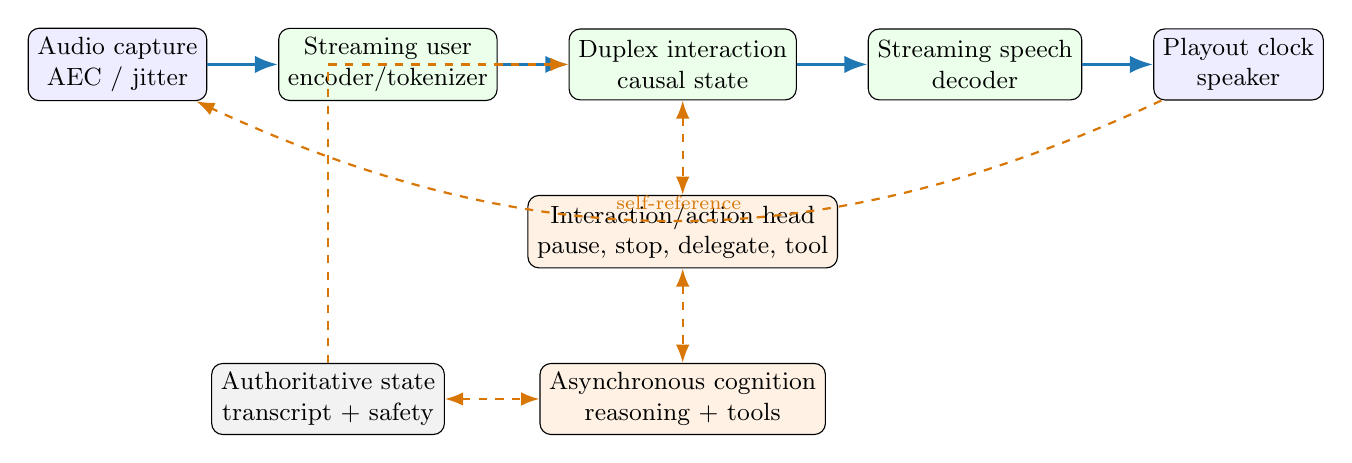
\begin{tikzpicture}[>=Latex,node distance=7mm and 9mm,font=\small,
box/.style={draw,rounded corners,align=center,minimum height=9mm},
f/.style={->,very thick,official},e/.style={->,thick,dashed,hypothesis}]
\node[box,fill=blue!7] (mic) {Audio capture\\AEC / jitter};
\node[box,fill=green!8,right=of mic] (enc) {Streaming user\\encoder/tokenizer};
\node[box,fill=green!8,right=of enc] (core) {Duplex interaction\\causal state};
\node[box,fill=green!8,right=of core] (dec) {Streaming speech\\decoder};
\node[box,fill=blue!7,right=of dec] (play) {Playout clock\\speaker};
\node[box,fill=orange!10,below=12mm of core] (action) {Interaction/action head\\pause, stop, delegate, tool};
\node[box,fill=orange!10,below=12mm of action] (frontier) {Asynchronous cognition\\reasoning + tools};
\node[box,fill=gray!10,left=12mm of frontier] (state) {Authoritative state\\transcript + safety};
\draw[f] (mic)--(enc); \draw[f] (enc)--(core); \draw[f] (core)--(dec); \draw[f] (dec)--(play);
\draw[e] (play) to[bend left=25] node[above,font=\scriptsize]{self-reference}(mic);
\draw[e,<->] (core)--(action); \draw[e,<->] (action)--(frontier); \draw[e,<->] (state)--(frontier); \draw[e] (state)|-(core);
\end{tikzpicture}%
}
\caption{Minimal architectural reconstruction that enables GPT-Live's public behavior. The green internal structure of speech and the orange action head are hypothetical; what is officially confirmed are continuous interaction, asynchronous delegation and system boundaries.}
\label{en:fig:reconstruction}
\end{figure}

\subsection{"Hybrid architecture" is more accurate than "pure end-to-end"}

On the perceptual -- vocalization path, end-to-end learning can preserve prosody, overlap, and non-verbal signals; on the complex task path, modular delegation allows the use of stronger reasoning models, tool permissions, and independent scaling; at the transport/state layer, deterministic protocols and explicit state machines are still irreplaceable. Therefore, GPT-Live is more like "an end-to-end interactive model embedded in a modular real-time system" rather than a single model annexation of all components.

This split also brings security and cost advantages: small and fast interactive models can be run frequently, and expensive models are only started when necessary; tool permissions are concentrated on the auditable cognitive plane; security controls can act on both real-time output and background results. The price is that cross-layer consistency, expired result processing, delegation strategies and session state recovery will be more complex.

\section{A reproducible open source implementation}

\subsection{Minimum Viable Architecture}

It is recommended to implement the research prototype as three independent services:

\begin{enumerate}
\item \textbf{Realtime gateway: }WebRTC ingress/egress, Opus, AEC/jitter buffer, playback timestamp, connection and weak network telemetry. Media packets go into bounded ring buffers, and application events go into reliable data channels.
\item \textbf{Duplex inference worker: } includes causal audio encoder, text LLM backbone, user-stream adapter, assistant audio decoder and action head. Workers maintain a fixed session affinity and perform an inference tick every 80 or 160 ms.
\item \textbf{Agent and state service: } are responsible for final transcription, conversation event log, tool runtime, reasoning model, context compaction, security policy and instance handoff coordination.
\end{enumerate}

The prototype can start from the voice backbone of the Moshi open source stack \cite{en:defossez2024moshi} and add independent action vocabulary and asynchronous tool bus; it can also adopt the Freeze-Omni/LSLM route, freeze the text LLM, and connect to the streaming encoder and lightweight audio decoder to reduce training costs \cite{en:wang2024freezeomni,en:ma2025lslm}. In the first stage, it is not appropriate to pursue video, long context, and multi-tool capabilities at the same time. The audio frame deadline and interruption behavior under real double-talk conditions should be verified first.

\subsection{Frame level scheduling pseudocode}

\begin{algorithm}[H]
\caption{Deadline-aware duplex session loop}
\begin{algorithmic}[1]
\ForAll{active session $s$ in earliest-deadline order}
  \State $u_t\gets$ readAudioChunk$(s,\Delta)$
  \State $e_t\gets$ drainReadyEvents$(s,\mathrm{contextEpoch})$
  \State $(a_t,z_t,m_t)\gets$ duplexStep$(u_t,e_t,m_{t-1})$
  \If{$z_t$ requests delegation and no equivalent task is active}
    \State enqueueAsync$(taskId,\mathrm{contextEpoch},\mathrm{query})$
  \EndIf
  \If{safety permits $a_t$ and playout deadline remains}
    \State sendAudio$(s,a_t,\mathrm{timestamp})$
  \Else
    \State applyGracefulDegradation$(s)$
  \EndIf
\EndFor
\State run background prefill, compaction, and telemetry with residual budget
\end{algorithmic}
\end{algorithm}

The scheduling loop needs to avoid three hidden blocking points: serial execution of the tokenizer or audio codec on the CPU; waiting for the final ASR transcript before updating the status; and incorrectly synchronously waiting for tool tasks in the media coroutine. All time-consuming operations should return results through events, and the media loop only consumes ready events.

\subsection{Phased experimental plan}

\paragraph{Phase A: Offline learnability}
Fixed 7B--9B text backbone and audio representation, and compared channel fusion, cross-attention and gated fusion under the condition that the number of training tokens is the same. The training set contains both half-duplex dialogue, synthetic overlap speech, and small-scale real binaural data. The acceptance criteria include: the degradation of spoke QA relative to the half-duplex baseline does not exceed the preset threshold; the recall of effective barge-in is improved and the false interruption rate does not deteriorate; self-trigger does not occur when echo exists.

\paragraph{Phase B: Single-machine real-time performance}
Gradually increase concurrent sessions on the fixed GPU, and record $Q/C$, DMR, P95/P99 jitter, KV cache memory and audio buffer underrun of each tick. Compare strategies such as FIFO, continuous batching, earliest deadline first (EDF), and reserved 20\% computing power. Acceptance is not based on the highest token throughput, but on the number of sessions that each GPU can stably carry.

\paragraph{Phase C: Asynchronous cognition}
Access a text reasoning model and three types of tools: low-latency query, long-latency search, and multi-round parameter completion. Compare the three modes of non-delegation, blocking delegation and asynchronous delegation, and check the tool result accuracy rate, interaction pauses, result expiration rate, computing power waste after task cancellation, and the user's subjective waiting experience.

\paragraph{Phase D: Long sessions and failures}
Run long sessions of 30, 60 and 120 minutes, actively injecting instance restart, network handoff, context compaction, transcript revision and tool-result race. The acceptance criteria include: there will be no duplication or deletion of speech during instance handoff; the context epoch will remain consistent; key user facts will be retained; and the GPU memory will not grow infinitely with the session duration.

\subsection{Resource and latency budget example}

When 160 ms is used as an inference tick, the following reference budget can be used: uplink and jitter buffer 40 ms, streaming encoder 15 ms, interaction backbone queuing and compute 45 ms, audio head and codec 20 ms, downlink, jitter buffer and playout 40 ms. This is not a public parameter of GPT-Live, just a starting point for engineering. Budgets must be verified using P95/P99 instead of average, and retested across geographies, low-end clients, and 5\% burst loss.

The cost model should be broken down by session minutes into interaction GPU, cognition GPU, audio bandwidth, tool calls, and idle reservation. If the delegation rate is $p_d$, the average reasoning time is $T_r$, and the interactive core cost per minute is $C_f$, the rough cost is
\begin{equation}
C_{min}=C_f+p_dT_rC_s+C_{net}+C_{tool}+C_{idle}.
\end{equation}
Reducing $p_d$ can save costs, but may also hurt task accuracy; therefore, it should be tuned together with delegation accuracy, recall, and final task success rate.

\section{Limitations, Open Questions, and Conclusions}

\subsection{Key details still unknown}

This report cannot determine GPT-Live's parameter count, training data, codec, audio-token rate, fusion-layer placement, use of joint action tokens, echo-reference injection, inference parallelism, or deployment scale because OpenAI has not publicly disclosed these details. Figure~\ref{en:fig:reconstruction} is a minimal implementation consistent with the publicly described behavior, not a leak or a reverse-engineering result.

It is also difficult to fairly compare existing papers. Moshi's "~200 ms", Neural-FSM's "response within 500 ms", GPT-4o's "average 320 ms" using different tasks, networks, hardware and latency starting points. This article reserves these numbers to illustrate their respective design goals and does not rank them into a unified ranking.

\subsection{Research Frontiers}

The most noteworthy directions in the future include: (1) adaptively selecting user-stream routing between strong semantic integration and resistance to overlap interference; (2) placing speech, language and action on a unified clock while avoiding high-frequency acoustic tokens from overwhelming sparse actions; (3) using real binaural data to train models that can adapt to different cultural turn-taking habits; (4) establishing factual fidelity and reversible audit mechanisms for long session compaction; (5) jointly optimizing inference tick, GPU scheduling, network jitter and playout clock; (6) Establish an asynchronous delegation benchmark covering stale result, task cancellation and provenance tracking.

\subsection{Conclusion}

The core of GPT-Live is not a mysterious acoustic module, but the reconstruction of a voice agent into a continuously running real-time system. Compared with the round-based full-modal model, it allows new inputs to continuously enter the model state during generation and synchronizes the interaction strategy with the real time; compared with the early single-model full-duplex solution, it further puts complex cognitive tasks into asynchronous paths for processing, and through stateful reasoning services, background context compression and instance switching, and low round-trip latency WebRTC, the model capabilities are transformed into a stable product experience.

Therefore, reproducing GPT-Live should not start with "training a larger speech LLM" starts, four closed loops should be established at the same time: \textbf{ represents the closed loop } to ensure that speaking and listening can be done in parallel, \textbf{ controls the closed loop } learning pause With interruption, \textbf{ cognitive closed loop } safely performs asynchronous delegation, \textbf{ system closed loop } ensures that each audio frame can arrive before the playback time limit. Public papers have given out most of the candidate mechanisms for these components; what is really difficult and most valuable for research is to make them collaborate stably in the same online system.

{\footnotesize
\begin{thebibliography}{38}
\providecommand{\natexlab}[1]{#1}
\providecommand{\url}[1]{\texttt{#1}}
\expandafter\ifx\csname urlstyle\endcsname\relax
  \providecommand{\doi}[1]{doi: #1}\else
  \providecommand{\doi}{doi: \begingroup \urlstyle{rm}\Url}\fi

\bibitem[{OpenAI}(2026{\natexlab{a}})]{en:openai2026continuous}
{OpenAI}.
\newblock How we built a realtime system for responsive voice {AI} in six
  months, August 2026{\natexlab{a}}.
\newblock URL
  \url{https://openai.com/index/continuous-voice-interaction-with-gpt-live/}.
\newblock Accessed 2026-08-07.

\bibitem[{OpenAI}(2026{\natexlab{b}})]{en:openai2026gptlive}
{OpenAI}.
\newblock Introducing {GPT-Live}, August 2026{\natexlab{b}}.
\newblock URL \url{https://openai.com/index/introducing-gpt-live/}.
\newblock Accessed 2026-08-07.

\bibitem[{OpenAI}(2024)]{en:openai2024gpt4osystemcard}
{OpenAI}.
\newblock {GPT-4o} system card, August 2024.
\newblock URL \url{https://openai.com/index/gpt-4o-system-card/}.
\newblock Accessed 2026-08-07.

\bibitem[Xu et~al.(2025)Xu, Guo, He, Hu, He, Bai, Chen, Wang, Fan, Dang, Zhang,
  Wang, Chu, and Lin]{en:xu2025qwenomni}
Jin Xu, Zhifang Guo, Jinzheng He, Hangrui Hu, Ting He, Shuai Bai, Keqin Chen,
  Jialin Wang, Yang Fan, Kai Dang, Bin Zhang, Xiong Wang, Yunfei Chu, and
  Junyang Lin.
\newblock {Qwen2.5-Omni} technical report.
\newblock \emph{arXiv preprint arXiv:2503.20215}, 2025.
\newblock URL \url{https://arxiv.org/abs/2503.20215}.

\bibitem[Zeng et~al.(2024)Zeng, Du, Liu, Wang, Jiang, Zhao, Dong, and
  Tang]{en:zeng2024glm4voice}
Aohan Zeng, Zhengxiao Du, Mingdao Liu, Kedong Wang, Shengmin Jiang, Lei Zhao,
  Yuxiao Dong, and Jie Tang.
\newblock {GLM-4-Voice}: Towards intelligent and human-like end-to-end spoken
  chatbot.
\newblock \emph{arXiv preprint arXiv:2412.02612}, 2024.
\newblock URL \url{https://arxiv.org/abs/2412.02612}.

\bibitem[Xie and Wu(2024)]{en:xie2024miniomni}
Zhifei Xie and Changqiao Wu.
\newblock Mini-omni: Language models can hear, talk while thinking in
  streaming.
\newblock \emph{arXiv preprint arXiv:2408.16725}, 2024.
\newblock URL \url{https://arxiv.org/abs/2408.16725}.

\bibitem[D{\'e}fossez et~al.(2024)D{\'e}fossez, Mazar{\'e}, Orsini, Royer,
  P{\'e}rez, J{\'e}gou, Grave, and Zeghidour]{en:defossez2024moshi}
Alexandre D{\'e}fossez, Laurent Mazar{\'e}, Manu Orsini, Am{\'e}lie Royer,
  Patrick P{\'e}rez, Herv{\'e} J{\'e}gou, Edouard Grave, and Neil Zeghidour.
\newblock Moshi: A speech-text foundation model for real-time dialogue.
\newblock \emph{arXiv preprint arXiv:2410.00037}, 2024.
\newblock URL \url{https://arxiv.org/abs/2410.00037}.

\bibitem[Veluri et~al.(2024)Veluri, Peloquin, Yu, Gong, and
  Gollakota]{en:veluri2024syncllm}
Bandhav Veluri, Benjamin~N. Peloquin, Bokai Yu, Hongyu Gong, and Shyamnath
  Gollakota.
\newblock Beyond turn-based interfaces: Synchronous {LLM}s as full-duplex
  dialogue agents.
\newblock In \emph{Proceedings of EMNLP}, pages 21390--21402, 2024.
\newblock \doi{10.18653/v1/2024.emnlp-main.1192}.
\newblock URL \url{https://aclanthology.org/2024.emnlp-main.1192/}.

\bibitem[Ma et~al.(2025)Ma, Song, Du, Cong, Chen, Wang, Wang, and
  Chen]{en:ma2025lslm}
Ziyang Ma, Yakun Song, Chenpeng Du, Jian Cong, Zhuo Chen, Yuping Wang, Yuxuan
  Wang, and Xie Chen.
\newblock Language model can listen while speaking.
\newblock In \emph{Proceedings of the AAAI Conference on Artificial
  Intelligence}, 2025.
\newblock URL \url{https://arxiv.org/abs/2408.02622}.

\bibitem[Wang et~al.(2024{\natexlab{a}})Wang, Lu, Tang, Yan, Xia, and
  Xiong]{en:wang2024neuralfsm}
Peng Wang, Songshuo Lu, Yaohua Tang, Sijie Yan, Wei Xia, and Yuanjun Xiong.
\newblock A full-duplex speech dialogue scheme based on large language model.
\newblock In \emph{Advances in Neural Information Processing Systems},
  volume~37, 2024{\natexlab{a}}.
\newblock URL
  \url{https://proceedings.neurips.cc/paper_files/paper/2024/hash/180d4373aca26bd86bf45fc50d1a709f-Abstract-Conference.html}.

\bibitem[Huang et~al.(2026)Huang, Zhang, Yu, Shi, Ma, Xu, Gao, Hao, He, and
  Liu]{en:huang2026duplexomni}
Muye Huang, Lingling Zhang, Xingyu Yu, Lei Shi, Zhanyu Ma, Jun Xu, Jiuchong
  Gao, Jinghua Hao, Renqing He, and Jun Liu.
\newblock Duplexomni: Real-time listening, seeing, thinking, and speaking for
  full-duplex interaction.
\newblock \emph{arXiv preprint arXiv:2606.09186}, 2026.
\newblock URL \url{https://arxiv.org/abs/2606.09186}.

\bibitem[{OpenAI}(2026{\natexlab{c}})]{en:openai2026safety}
{OpenAI}.
\newblock {GPT-Live} system card, August 2026{\natexlab{c}}.
\newblock URL \url{https://deploymentsafety.openai.com/gpt-live}.
\newblock Accessed 2026-08-07.

\bibitem[Vaswani et~al.(2017)Vaswani, Shazeer, Parmar, Uszkoreit, Jones, Gomez,
  Kaiser, and Polosukhin]{en:vaswani2017attention}
Ashish Vaswani, Noam Shazeer, Niki Parmar, Jakob Uszkoreit, Llion Jones,
  Aidan~N. Gomez, Lukasz Kaiser, and Illia Polosukhin.
\newblock Attention is all you need.
\newblock In \emph{Advances in Neural Information Processing Systems},
  volume~30, 2017.
\newblock URL \url{https://arxiv.org/abs/1706.03762}.

\bibitem[Zhang et~al.(2026)Zhang, Chen, Wu, Li, Zhang, Zhang, Liu, Lin, Peng,
  Liu, Chng, Yan, Wu, Huang, Yang, and Tian]{en:zhang2026duplexsla}
Haoyang Zhang, Jun Chen, Donghang Wu, Yuxin Li, Yuxin Zhang, Xiangyu~Tony
  Zhang, Che Liu, Qingjian Lin, Yizhou Peng, Hexin Liu, Eng~Siong Chng, Chao
  Yan, Boyong Wu, Yechang Huang, Xuerui Yang, and Fei Tian.
\newblock Duplexsla: A full-duplex spoken language model with synchronized
  speech, language, and action.
\newblock \emph{arXiv preprint arXiv:2605.20755}, 2026.
\newblock URL \url{https://arxiv.org/abs/2605.20755}.

\bibitem[Yu et~al.(2025)Yu, Wang, Yang, Chen, Tian, Zhang, Sun, Lu, Wang, and
  Zhang]{en:yu2025salmonnomni}
Wenyi Yu, Siyin Wang, Xiaoyu Yang, Xianzhao Chen, Xiaohai Tian, Jun Zhang,
  Guangzhi Sun, Lu~Lu, Yuxuan Wang, and Chao Zhang.
\newblock {SALMONN}-omni: A standalone speech {LLM} without codec injection for
  full-duplex conversation.
\newblock In \emph{Advances in Neural Information Processing Systems},
  volume~38, 2025.
\newblock URL
  \url{https://proceedings.neurips.cc/paper_files/paper/2025/hash/233aee920dab065709145371b5900b8f-Abstract-Conference.html}.

\bibitem[Zeghidour et~al.(2022)Zeghidour, Luebs, Omran, Skoglund, and
  Tagliasacchi]{en:zeghidour2021soundstream}
Neil Zeghidour, Alejandro Luebs, Ahmed Omran, Jan Skoglund, and Marco
  Tagliasacchi.
\newblock Soundstream: An end-to-end neural audio codec.
\newblock \emph{IEEE/ACM Transactions on Audio, Speech, and Language
  Processing}, 30:\penalty0 495--507, 2022.
\newblock URL \url{https://arxiv.org/abs/2107.03312}.

\bibitem[D{\'e}fossez et~al.(2022)D{\'e}fossez, Copet, Synnaeve, and
  Adi]{en:defossez2022encodec}
Alexandre D{\'e}fossez, Jade Copet, Gabriel Synnaeve, and Yossi Adi.
\newblock High fidelity neural audio compression.
\newblock \emph{arXiv preprint arXiv:2210.13438}, 2022.
\newblock URL \url{https://arxiv.org/abs/2210.13438}.

\bibitem[Borsos et~al.(2022)Borsos, Marinier, Vincent, Kharitonov, Pietquin,
  Sharifi, Roblek, Teboul, Grangier, Tagliasacchi, and
  Zeghidour]{en:borsos2022audiolm}
Zal{\'a}n Borsos, Rapha{\"e}l Marinier, Damien Vincent, Eugene Kharitonov,
  Olivier Pietquin, Matt Sharifi, Dominik Roblek, Olivier Teboul, David
  Grangier, Marco Tagliasacchi, and Neil Zeghidour.
\newblock {AudioLM}: A language modeling approach to audio generation.
\newblock \emph{arXiv preprint arXiv:2209.03143}, 2022.
\newblock URL \url{https://arxiv.org/abs/2209.03143}.

\bibitem[Long et~al.(2025)Long, Shen, Fu, Gao, Li, Chen, Zhang, Shao, Li, Peng,
  Cao, Li, Ji, and Sun]{en:long2025vitaaudio}
Zuwei Long, Yunhang Shen, Chaoyou Fu, Heting Gao, Lijiang Li, Peixian Chen,
  Mengdan Zhang, Hang Shao, Jian Li, Jinlong Peng, Haoyu Cao, Ke~Li, Rongrong
  Ji, and Xing Sun.
\newblock {VITA-Audio}: Fast interleaved cross-modal token generation for
  efficient large speech-language model.
\newblock \emph{arXiv preprint arXiv:2505.03739}, 2025.
\newblock URL \url{https://arxiv.org/abs/2505.03739}.

\bibitem[Chen and Yu(2025)]{en:chen2025survey}
Yuxuan Chen and Haoyuan Yu.
\newblock From turn-taking to synchronous dialogue: A survey of full-duplex
  spoken language models.
\newblock \emph{arXiv preprint arXiv:2509.14515}, 2025.
\newblock URL \url{https://arxiv.org/abs/2509.14515}.

\bibitem[Zhang et~al.(2024)Zhang, Cheng, Deng, Chen, Wang, Zheng, Liu, Yu, Tan,
  Du, and Zhang]{en:zhang2024omniflatten}
Qinglin Zhang, Luyao Cheng, Chong Deng, Qian Chen, Wen Wang, Siqi Zheng,
  Jiaqing Liu, Hai Yu, Chaohong Tan, Zhihao Du, and Shiliang Zhang.
\newblock Omniflatten: An end-to-end {GPT} model for seamless voice
  conversation.
\newblock \emph{arXiv preprint arXiv:2410.17799}, 2024.
\newblock URL \url{https://arxiv.org/abs/2410.17799}.

\bibitem[Nguyen et~al.(2022)Nguyen, Kharitonov, Copet, Adi, Hsu, Elkahky,
  Tomasello, Algayres, Sagot, Mohamed, and Dupoux]{en:nguyen2022dgslm}
Tu~Anh Nguyen, Eugene Kharitonov, Jade Copet, Yossi Adi, Wei-Ning Hsu, Ali
  Elkahky, Paden Tomasello, Robin Algayres, Benoit Sagot, Abdelrahman Mohamed,
  and Emmanuel Dupoux.
\newblock Generative spoken dialogue language modeling.
\newblock \emph{arXiv preprint arXiv:2203.16502}, 2022.
\newblock URL \url{https://arxiv.org/abs/2203.16502}.

\bibitem[Lu et~al.(2026)Lu, Chen, Wang, Peng, Kang, Wu, and Wu]{en:lu2026routing}
Hui Lu, Xueyuan Chen, Huimeng Wang, Shuhai Peng, Shiyin Kang, Xixin Wu, and
  Zhiyong Wu.
\newblock How should {LLM}s listen while speaking? a study of user-stream
  routing in full-duplex spoken dialogue.
\newblock \emph{arXiv preprint arXiv:2605.10199}, 2026.
\newblock URL \url{https://arxiv.org/abs/2605.10199}.

\bibitem[Nakata et~al.(2026)Nakata, Saito, and
  Saruwatari]{en:nakata2026duplexchat}
Wataru Nakata, Yuki Saito, and Hiroshi Saruwatari.
\newblock Duplexchat: Constructing speaker-separated full-duplex dialogue
  speech at scale for spoken dialogue language modeling.
\newblock \emph{arXiv preprint arXiv:2607.04941}, 2026.
\newblock URL \url{https://arxiv.org/abs/2607.04941}.

\bibitem[Wang et~al.(2024{\natexlab{b}})Wang, Li, Fu, Shen, Xie, Li, Sun, and
  Ma]{en:wang2024freezeomni}
Xiong Wang, Yangze Li, Chaoyou Fu, Yunhang Shen, Lei Xie, Ke~Li, Xing Sun, and
  Long Ma.
\newblock Freeze-omni: A smart and low latency speech-to-speech dialogue model
  with frozen {LLM}.
\newblock \emph{arXiv preprint arXiv:2411.00774}, 2024{\natexlab{b}}.
\newblock URL \url{https://arxiv.org/abs/2411.00774}.

\bibitem[Dai et~al.(2019)Dai, Yang, Yang, Carbonell, Le, and
  Salakhutdinov]{en:dai2019transformerxl}
Zihang Dai, Zhilin Yang, Yiming Yang, Jaime Carbonell, Quoc~V. Le, and Ruslan
  Salakhutdinov.
\newblock Transformer-{XL}: Attentive language models beyond a fixed-length
  context.
\newblock \emph{arXiv preprint arXiv:1901.02860}, 2019.
\newblock URL \url{https://arxiv.org/abs/1901.02860}.

\bibitem[Kwon et~al.(2023)Kwon, Li, Zhuang, Sheng, Zheng, Yu, Gonzalez, Zhang,
  and Stoica]{en:kwon2023pagedattention}
Woosuk Kwon, Zhuohan Li, Siyuan Zhuang, Ying Sheng, Lianmin Zheng, Cody~Hao Yu,
  Joseph~E. Gonzalez, Hao Zhang, and Ion Stoica.
\newblock Efficient memory management for large language model serving with
  {PagedAttention}.
\newblock In \emph{Proceedings of the ACM Symposium on Operating Systems
  Principles}, 2023.
\newblock URL \url{https://arxiv.org/abs/2309.06180}.

\bibitem[Dao et~al.(2022)Dao, Fu, Ermon, Rudra, and
  R{\'e}]{en:dao2022flashattention}
Tri Dao, Daniel~Y. Fu, Stefano Ermon, Atri Rudra, and Christopher R{\'e}.
\newblock {FlashAttention}: Fast and memory-efficient exact attention with
  {IO}-awareness.
\newblock In \emph{Advances in Neural Information Processing Systems},
  volume~35, 2022.
\newblock URL \url{https://arxiv.org/abs/2205.14135}.

\bibitem[Leviathan et~al.(2023)Leviathan, Kalman, and
  Matias]{en:leviathan2023speculative}
Yaniv Leviathan, Matan Kalman, and Yossi Matias.
\newblock Fast inference from transformers via speculative decoding.
\newblock In \emph{Proceedings of ICML}, 2023.
\newblock URL \url{https://arxiv.org/abs/2211.17192}.

\bibitem[Alvestrand(2021)]{en:alvestrand2021webrtc}
Harald Alvestrand.
\newblock Overview: Real-time protocols for browser-based applications.
\newblock Technical Report RFC 8825, Internet Engineering Task Force, 2021.
\newblock URL \url{https://datatracker.ietf.org/doc/rfc8825/}.

\bibitem[Jesup et~al.(2021)Jesup, Loreto, and T{\"u}xen]{en:jesup2021datachannels}
Randell Jesup, Salvatore Loreto, and Michael T{\"u}xen.
\newblock {WebRTC} data channels.
\newblock Technical Report RFC 8831, Internet Engineering Task Force, 2021.
\newblock URL \url{https://datatracker.ietf.org/doc/rfc8831/}.

\bibitem[Agranovich et~al.(2024)Agranovich, Nachmani, Rybakov, Ding, Jia, Bar,
  Zen, and Ramanovich]{en:agranovich2024simultron}
Alex Agranovich, Eliya Nachmani, Oleg Rybakov, Yifan Ding, Ye~Jia, Nadav Bar,
  Heiga Zen, and Michelle~Tadmor Ramanovich.
\newblock Simultron: On-device simultaneous speech-to-speech translation.
\newblock \emph{arXiv preprint arXiv:2406.02133}, 2024.
\newblock URL \url{https://arxiv.org/abs/2406.02133}.

\bibitem[Rescorla et~al.(2022)Rescorla, Tschofenig, and
  Modadugu]{en:rescorla2022dtls13}
Eric Rescorla, Hannes Tschofenig, and Nagendra Modadugu.
\newblock The datagram transport layer security ({DTLS}) protocol version 1.3.
\newblock Technical Report RFC 9147, Internet Engineering Task Force, 2022.
\newblock URL \url{https://datatracker.ietf.org/doc/rfc9147/}.

\bibitem[Hancke et~al.(2026)Hancke, Rescorla, and Rose]{en:hancke2026sped}
Philipp Hancke, Eric Rescorla, and Jonny Rose.
\newblock {SPED}: {STUN} protocol for embedding {DTLS}.
\newblock Technical Report draft-hancke-webrtc-sped-00, Internet Engineering
  Task Force, 2026.
\newblock URL \url{https://datatracker.ietf.org/doc/draft-hancke-webrtc-sped/}.
\newblock Internet-Draft, work in progress.

\bibitem[Hancke and Rescorla(2026)]{en:hancke2026snap}
Philipp Hancke and Eric Rescorla.
\newblock {SNAP}: Accelerating {WebRTC} data channel establishment.
\newblock Technical Report draft-hancke-tsvwg-snap-00, Internet Engineering
  Task Force, 2026.
\newblock URL \url{https://datatracker.ietf.org/doc/draft-hancke-tsvwg-snap/}.
\newblock Internet-Draft, work in progress.

\bibitem[Lin et~al.(2025)Lin, Lian, Li, Wang, Anumanchipalli, Liu, and
  Lee]{en:lin2025fullduplexbench}
Guan-Ting Lin, Jiachen Lian, Tingle Li, Qirui Wang, Gopala Anumanchipalli,
  Alexander~H. Liu, and Hung-yi Lee.
\newblock Full-duplex-bench: A benchmark to evaluate full-duplex spoken
  dialogue models on turn-taking capabilities.
\newblock \emph{arXiv preprint arXiv:2503.04721}, 2025.
\newblock URL \url{https://arxiv.org/abs/2503.04721}.

\bibitem[Lin et~al.(2026)Lin, Kuan, Shi, Chang, Arora, Watanabe, and
  Lee]{en:lin2026fullduplexbenchv2}
Guan-Ting Lin, Shih-Yun~Shan Kuan, Jiatong Shi, Kai-Wei Chang, Siddhant Arora,
  Shinji Watanabe, and Hung-yi Lee.
\newblock Full-duplex-bench-v2: A multi-turn evaluation framework for duplex
  dialogue systems with an automated examiner.
\newblock In \emph{Proceedings of ACL}, 2026.
\newblock URL \url{https://aclanthology.org/2026.acl-short.4/}.

\bibitem[Stivers et~al.(2009)Stivers, Enfield, Brown, Englert, Hayashi,
  Heinemann, Hoymann, Rossano, de~Ruiter, Yoon, and
  Levinson]{en:stivers2009turntaking}
Tanya Stivers, N.~J. Enfield, Penelope Brown, Christina Englert, Makoto
  Hayashi, Trine Heinemann, Gertie Hoymann, Federico Rossano, Jan~Peter
  de~Ruiter, Kyung-Eun Yoon, and Stephen~C. Levinson.
\newblock Universals and cultural variation in turn-taking in conversation.
\newblock \emph{Proceedings of the National Academy of Sciences}, 106\penalty0
  (26):\penalty0 10587--10592, 2009.
\newblock \doi{10.1073/pnas.0903616106}.

\end{thebibliography}
}
\clearpage
\pdfbookmark[0]{中文版}{bilingual.chinese}
\setcounter{section}{0}
\setcounter{subsection}{0}
\setcounter{subsubsection}{0}
\setcounter{equation}{0}
\setcounter{figure}{0}
\setcounter{table}{0}
\setcounter{footnote}{0}
\setcounter{tocdepth}{2}
\renewcommand{\abstractname}{摘要}
\renewcommand{\contentsname}{目录}
\renewcommand{\figurename}{图}
\renewcommand{\tablename}{表}
\renewcommand{\refname}{参考文献}
\renewcommand{\appendixname}{附录}
\BilingualUseChineseToc
\renewcommand*{\theHsection}{zh.\arabic{section}}
\renewcommand*{\theHsubsection}{zh.\arabic{section}.\arabic{subsection}}
\renewcommand*{\theHsubsubsection}{zh.\arabic{section}.\arabic{subsection}.\arabic{subsubsection}}
\renewcommand*{\theHequation}{zh.\arabic{equation}}
\renewcommand*{\theHfigure}{zh.\arabic{figure}}
\renewcommand*{\theHtable}{zh.\arabic{table}}
\gdef\BilingualAnchorPrefix{zh}
\fancyhead[L]{\small\color{gray}GPT-Live 技术架构推演}
\markboth{}{}
\begin{center}
  {\zihao{2}\bfseries\color{navy} 一文详解 GPT-Live：基于公开资料的技术架构推演与实现设想}\par
  \vspace{4pt}
  {\zihao{3}\color{navy} 全双工连续推理架构相关技术}\par
  \vspace{10pt}
  {\normalsize\textbf{Jiguo Li\footnote{本文在 OpenAI Codex 的协助下完成。}}}\par
  \vspace{2pt}
  {\small\href{mailto:jiguolee@gmail.com}{jiguolee@gmail.com}}\par
  \vspace{2pt}
  {\small 2026 年 8 月}
\end{center}
\vspace{5pt}
\hrule

\begin{abstract}
截至本文写作时，OpenAI 尚未发布 GPT-Live 的完整技术报告，也未公开其具体模型结构、音频表示、训练数据与训练方法等实现细节。因此，本文并非对 OpenAI 官方技术报告或内部实现的复述，而是基于公开材料所作的技术推演。本文缘起于 OpenAI 近期发布的一篇 GPT-Live 工程博客：该文披露了系统从轮次式交互转向 continuous inference 的若干系统级设计，包括异步委派、有状态实例切换和低时延传输，由此引发了笔者对其可能实现路径的兴趣。本文以这些已披露的系统边界为起点，结合 OpenAI 官方工程说明、系统卡、Internet Engineering Task Force（IETF）协议草案，以及 2024--2026 年全双工语音模型论文与开源项目，重建一套技术上可行、但未经 OpenAI 证实的参考架构。其核心判断是：若要实现 GPT-Live 所展示的能力，系统不能只依赖“更强的端到端 speech-to-speech model”，还需要全双工交互核心、异步认知委派、stateful serving 和低往返时延实时传输的协同。本文进一步形式化 continuous inference，比较 codec token、codec-free、双流融合、cross-attention、finite-state machine control token 与 action channel 等公开路线；分析训练数据、长会话状态、attention cache、上下文压缩、故障切换和 WebRTC/WARP；最后给出可复现的开源实现设想、消融实验与多维评测体系。文中引用的公开论文和开源项目仅用于说明可能的实现机制，不能据此认定 GPT-Live 采用了相同设计。全文使用 \FOne 官方事实、\FTwo 公开机制和 \Hyp 推断性重建三级证据标签，以区分已披露事实与作者推演。

\noindent\textbf{关键词：}GPT-Live；全双工语音模型；continuous inference；speech-to-speech；实时系统；WebRTC；stateful serving
\end{abstract}

\noteBox{\textbf{阅读提要：}GPT-Live 的关键不只是一个端到端 speech-to-speech model，而是 full-duplex interaction core、异步 cognition、stateful serving 与低延迟实时传输的协同。}

\clearpage
\begingroup
\small
\setlength{\parskip}{0pt}
\linespread{1.02}\selectfont
\setcounter{tocdepth}{2}
\tableofcontents
\endgroup
\clearpage

\section{问题定义、证据边界与演进路线}

\subsection{研究缘起：从 OpenAI 的一篇工程博客说起}

本文的直接缘起，是 OpenAI 于 2026 年 8 月 3 日发布的工程博客《How We Built a Realtime System for Responsive Voice AI in Six Months》\cite{zh:openai2026continuous}。与通常侧重功能展示和评测结果的产品介绍不同，这篇文章从工程实现出发，解释了团队为何放弃依赖轮次检测器的传统语音架构，以及如何在六个月内重新设计推理、上下文管理和媒体传输系统。博客披露的若干细节尤其引起了笔者的兴趣：语音模型可以同时听和说；媒体帧通过独立的快速路径传输；复杂推理和工具调用沿另一条异步路径执行；长会话通过后台上下文压缩和模型实例切换保持连续；WARP 与 Instant Connect 则试图进一步缩短 WebRTC\footnote{Web Real-Time Communication，Web 实时通信技术栈，用于浏览器或客户端之间的低延迟音视频与数据传输。} 建连时间。

这些公开信息勾勒出了 GPT-Live 的系统轮廓，却也留下了更值得追问的问题：全双工语音模型如何在生成期间持续接收新输入？模型如何表示双方重叠的语音以及暂停、简短应答和打断等交互动作？快速交互模型与深层推理模型之间如何传递上下文和结果？一个持续数十分钟的有状态会话，又如何在 GPU 调度、KV 缓存、网络抖动和实例故障之下保持流畅？

这篇博客因此成为本文的出发点。本文并不复述其产品功能，而是以其中公开的系统边界为线索，结合近几年的顶会论文、技术报告、开源实现和网络协议，尝试还原一套技术上自洽、证据上可追溯的 GPT-Live 架构图景。换言之，本文要回答的不只是“GPT-Live 有哪些能力”，而是“为了实现这些能力，模型与系统分别需要解决什么问题”。

\subsection{本文究竟解释什么}

“GPT-Live 如何实现”包含两个容易混淆的问题。其一是\emph{模型问题}：音频如何表示，用户流如何进入 Transformer，模型如何同时预测语义、声学与交互动作。其二是\emph{系统问题}：网络抖动、连续会话、GPU 推理时限、KV 缓存、复杂推理与工具调用如何在不中断语音交互的条件下协同工作。GPT-Live 的公开材料表明，系统问题已经与模型问题同等重要\cite{zh:openai2026gptlive,zh:openai2026continuous}。因此，本文研究的是“能够处理自然语音重叠、随时接受打断、持续反馈并执行后台任务的在线语音智能体”，而不是某个孤立的模型检查点。

证据采用三级标注：\FOne 仅来自 OpenAI 官方文章和系统卡；\FTwo 来自同行评审论文、作者技术报告、开源代码或标准；\Hyp 是由多项事实共同约束的架构重建。尤其需要强调，OpenAI 没有公开 GPT-Live 的参数量、音频 tokenizer、frame rate、attention 连接方式、训练 token 数或集群规模。Moshi、DuplexOmni 等工作可以说明一种机制在工程上可行，却不能证明 GPT-Live 使用同一机制。

\subsection{四代语音交互范式}

\paragraph{级联式语音管线。}
传统系统串联 VAD/endpointing、ASR、文本 LLM 和 TTS\footnote{VAD：Voice Activity Detection，语音活动检测；ASR：Automatic Speech Recognition，自动语音识别；LLM：Large Language Model，大语言模型；TTS：Text-to-Speech，文本转语音。}。其优势是模块可观测、组件易替换、文本工具生态成熟；问题是误差逐层累积，韵律与非语言信号在文本瓶颈处丢失，而且每轮必须等待“用户说完”。总延迟可粗略写为
\begin{equation}
T_{\mathrm{cascade}}=T_{\mathrm{endpoint}}+T_{\mathrm{ASR}}+T_{\mathrm{LLM,first}}+T_{\mathrm{TTS,first}}+T_{\mathrm{net}}.
\end{equation}
其中，端点检测（endpointing）往往是尾部延迟的主要来源。即便所有模型都支持流式处理，只要状态机仍强制各模块串行运行，交互本质上仍是半双工。

\paragraph{轮次式端到端 Omni Model。}
GPT-4o 将文本、视觉和音频统一到一个神经网络中，官方报告其音频响应最低可达 $232\ms$、平均为 $320\ms$\cite{zh:openai2024gpt4osystemcard}。\FOne 这种架构缓解了级联管线中的模态信息损失，并降低了部分首包延迟，但“端到端”并不自然等同于“全双工”：如果推理 API\footnote{Application Programming Interface，应用程序编程接口。} 在生成期间不再接收新的用户音频帧，或仍依赖外部 VAD 判定一轮对话结束，系统依然是轮次式的。Qwen2.5-Omni 的 Thinker--Talker、GLM-4-Voice 与 Mini-Omni 展示了流式语音到语音的不同实现\cite{zh:xu2025qwenomni,zh:zeng2024glm4voice,zh:xie2024miniomni}，但其交互调度能力仍需单独评估。

\paragraph{单模型全双工。}
Moshi、SyncLLM、LSLM 和 Neural-FSM 将时间以及用户、助手两条音频流显式纳入建模：同一时刻既有用户通道，也有助手通道，模型可以选择静默、给出简短应答、继续发言、停止或接受打断\cite{zh:defossez2024moshi,zh:veluri2024syncllm,zh:ma2025lslm,zh:wang2024neuralfsm}。此时，inference unit 从“一轮对话”缩短为固定时长的 audio frame 或 chunk；延迟关注点也从 time-to-first-token（TTFT），转变为每个 audio frame 能否在 playout deadline 前完成。

\paragraph{交互--认知解耦的连续智能体。}
\FOne GPT-Live 将快速交互与复杂思考拆开：交互模型持续监听和发声，深层推理或工具调用异步委派给更强模型；结果准备好后再自然并入对话\cite{zh:openai2026gptlive,zh:openai2026continuous}。2026 年 DuplexOmni 独立提出 interaction layer 与 pluggable thinking layer 的并行结构\cite{zh:huang2026duplexomni}，为这种范式提供公开学术参照。它不是回到 ASR--LLM--TTS 级联，而是让低延迟闭环与高智能闭环工作在不同时间尺度。

\begin{figure}[H]
\centering
\begin{tikzpicture}[node distance=6mm,>=Latex,font=\small,
box/.style={draw,rounded corners,minimum height=10mm,text width=31mm,align=center,fill=blue!5},
arr/.style={->,thick}]
\node[box] (c1) {级联语音\\VAD$\to$ASR\\LLM$\to$TTS};
\node[box,right=of c1] (c2) {Turn-based Omni\\统一模态，轮次推进};
\node[box,right=of c2] (c3) {Full-duplex Model\\双方流+统一时钟};
\node[box,right=of c3,fill=orange!10] (c4) {Continuous Agent\\交互层$\parallel$思考层};
\draw[arr] (c1)--(c2);
\draw[arr] (c2)--(c3);
\draw[arr] (c3)--(c4);
\end{tikzpicture}
\caption{语音模型的关键演进不是单纯扩大参数，而是逐步解除文本瓶颈、轮次屏障和单时间尺度推理。}
\label{zh:fig:evolution}
\end{figure}

\subsection{GPT-Live 的官方系统轮廓}

\FOne OpenAI 描述的线上系统可归纳为四个平面。第一，\textbf{媒体平面（media plane）}通过 WebRTC 持续收发音频，并处理 packet loss、jitter、clock drift 和 audio catch-up。第二，\textbf{交互平面（interaction plane）}运行 GPT-Live 语音模型，按照 audio clock 持续决定何时说、听、停、插话、调用工具或发起委派。第三，\textbf{认知平面（cognition plane）}维护预先创建和填充、具有稳定 session affinity 的 frontier-model session，用于承接复杂推理。第四，\textbf{控制与状态平面（control/state plane）}维护 session state、transcript、context compaction、安全控制和 instance handoff\cite{zh:openai2026continuous,zh:openai2026safety}。

在媒体快速路径与应用逻辑之间设置异步 RPC\footnote{Remote Procedure Call，远程过程调用。} 边界至关重要：数据库访问、业务逻辑或耗时工具都不能反向阻塞音频帧。系统因而存在两个一致性层级：音频路径采用“时限优先”的弱同步方式，应用状态则采用可重试的事件语义。连续音频之上仍可推导出离散的语义轮次，并同时维护临时转写（speculative transcript）和最终转写（authoritative transcript）。因此，“取消轮次检测器”指的是取消会阻塞音频路径的轮次门控，而不是放弃语义分段。

\begin{figure}[H]
\centering
\begin{tikzpicture}[>=Latex,node distance=8mm and 10mm,
p/.style={draw,rounded corners,minimum width=28mm,minimum height=10mm,align=center},
fast/.style={->,very thick,official},slow/.style={->,thick,dashed,hypothesis}]
\node[p,fill=blue!7] (client) {客户端\\Mic / Speaker};
\node[p,fill=blue!7,right=of client] (media) {Media Fast Path\\WebRTC / WARP};
\node[p,fill=green!8,right=of media] (live) {GPT-Live\\Interaction Core};
\node[p,fill=orange!10,right=16mm of live] (think) {Frontier Model\\Reasoning / Tools};
\node[p,fill=gray!10,below=12mm of live] (state) {Session State\\Transcript / Safety / Compaction};
\draw[fast,<->] (client)--(media);
\draw[fast,<->] (media)--(live);
\draw[slow,<->] (live)--node[above,font=\scriptsize]{async delegation}(think);
\draw[slow,<->] (live)--(state);
\draw[slow,<->] (think)|-(state);
\end{tikzpicture}
\caption{证据约束下的 GPT-Live 系统轮廓。蓝色实线是低延迟媒体闭环，橙色虚线是允许更高延迟的认知与状态闭环。图中逻辑分层来自官方事实；模块内部实现仍未公开。}
\label{zh:fig:official-architecture}
\end{figure}

\section{全双工连续推理的形式化}

轮次式 LLM 只需保证 token 序列上的因果性；full-duplex model 还必须保证每个 audio chunk 的排队与计算时间满足 $Q_t+C_t\leq\Delta$，否则即使语义正确，也会因错过 playout deadline 而产生卡顿。因而 continuous inference 的状态不仅包含历史语义，还必须同步用户音频、助手自身输出、播放进度、工具事件和安全信号，并让低延迟 interaction path 与高成本 cognition path 在不同时间尺度上并行推进。

\subsection{从 token 序列到受 wall-clock 约束的双流过程}

下述形式化以标准 Transformer 自回归建模为起点\cite{zh:vaswani2017attention}。

普通自回归 LLM 建模 $p(y_n\mid x,y_{<n})$，输入 $x$ 在解码开始前已经固定。全双工语音则不同：助手生成语音时，新的用户输入仍在持续到达。将 wall-clock 离散为长度为 $\Delta$ 的 audio chunk，令 $u_t$ 表示第 $t$ 个用户 audio chunk，$a_t$ 表示助手输出，$z_t$ 表示内部交互动作，$m_t$ 表示持久状态，则系统需要在每个 playout deadline 之前完成以下计算：
\begin{align}
m_t &= f_\theta(m_{t-1},u_t,\tilde a_{t-d:t-1},e_t),\\
(a_t,z_t) &\sim p_\theta(\cdot\mid m_t),\qquad
z_t\in\{\texttt{listen,speak,pause,stop,backchannel,delegate,tool}\}.
\end{align}
$\tilde a$ 表示系统自身的回放参考，或经过声学回声消除后的自身输出；$e_t$ 表示工具结果、网络状态和安全信号。这里最重要的约束不是概率公式本身，而是 $C_t+Q_t\leq\Delta$：单个 audio chunk 的计算时间 $C_t$ 与排队时间 $Q_t$ 之和必须小于 playout deadline。偶发超时会造成 audio underrun，连续超时则会表现为机械式停顿。

全双工至少包含四层含义：（1）传输层可同时上行和下行；（2）模型在发声时仍持续编码用户输入；（3）策略层能够处理语音重叠、简短应答和用户插话；（4）会话层在后台任务执行期间仍保持可交互。仅具备双向 WebSocket 连接并不能称为全双工模型；如果系统在处理复杂任务时冻结交互，即使具备前三层能力，也不等于 GPT-Live 所强调的连续智能体。

\subsection{状态、因果性与回声}

因果系统只能使用 $u_{\le t}$，但可通过有限 look-ahead $L$ 换取更稳健的语音表征。算法延迟下界近似为
\begin{equation}
T_{\mathrm{algo}}=T_{\mathrm{chunk}}+T_{\mathrm{lookahead}}+T_{\mathrm{codec}}+T_{\mathrm{decode}}.
\end{equation}
减小 $\Delta$ 会提高决策频率，却增加 token rate、kernel launch 与调度压力。以 80--160 ms 为时间格的公开系统体现了典型折中：足够快以响应打断，又能在一个格内积累可辨别的声学证据\cite{zh:defossez2024moshi,zh:zhang2026duplexsla}。

模型还必须区分“用户正在说”与“扬声器声音被麦克风重新采集”。传统 AEC\footnote{Acoustic Echo Cancellation，声学回声消除。} 在波形域消除已知播放参考；模型侧还可显式接收 assistant history、自输出 token 或 echo flag。若只用单通道混合音频训练，模型可能把自己的声音误当用户指令。SALMONN-omni 将 echo cancellation 列为全双工核心场景\cite{zh:yu2025salmonnomni}，说明评估必须覆盖残余回声、双讲与不同声学路径，而不能只在干净的分离声道上测试。

\subsection{双时间尺度控制}

自然对话的控制延迟与任务推理延迟并不相同。快速环 $\pi_f$ 每 $\Delta$ 毫秒运行，负责保持接触、决定是否让出话权；慢速环 $\pi_s$ 可能运行数秒，负责搜索、规划或调用工具：
\begin{equation}
\pi_f:(u_t,m_{t-1})\mapsto(a_t,z_t),\qquad
\pi_s:(q,M)\mapsto r,quad r\xrightarrow{\mathrm{event}}m_{t+k}.
\end{equation}
异步委派的难点在于如何将结果重新注入当前对话：结果可能已经过时，任务可能被用户取消，也可能与交互层先前的表述发生冲突。因此，事件至少应包含 \texttt{task\_id}、上下文版本、创建时间、取消状态和来源信息；交互层收到结果后还应执行相关性判断，而不是无条件朗读。

\section{公开模型路线：组件与设计轴}

近年的公开模型虽然实现路径不同，却逐渐收敛到“共享时间轴、用户与助手双流、持续状态更新”这一基本结构。真正影响系统行为的是三组权衡：codec token 的生成统一性与高 token rate，channel fusion 的语义耦合能力与 overlap 干扰，以及 silence/control/action token 的控制精度与主干负担；这些设计轴可以解释 Moshi、SyncLLM、LSLM、Neural-FSM 和 DuplexSLA 的差异，也构成理解 GPT-Live 的候选机制空间。

\subsection{音频表示：连续特征、semantic token 与 codec token}

端到端语音 LLM 通常先把 16/24 kHz 波形降采样为低频表示。SoundStream 与 EnCodec 使用卷积编码器、残差向量量化（RVQ）和生成式解码器，将波形压缩为多 codebook 离散 token\cite{zh:zeghidour2021soundstream,zh:defossez2022encodec}。若帧率为 $f$、codebook 数为 $K$、每本词表大小为 $V_k$，原始离散码率为
\begin{equation}
R=f\sum_{k=1}^{K}\log_2V_k\quad\text{bit/s}.
\end{equation}
高层 codebook 往往承载较粗的语义和韵律，后续 codebook 补充声学细节。AudioLM 进一步分离 semantic token 与 acoustic token，以较低频语义保证长期一致性，以 codec code 重建音质\cite{zh:borsos2022audiolm}。

VITA-Audio 用 multiple cross-modal token prediction 在一次 forward pass 中生成多个 audio token，作者报告 7B 规模下获得 3--5 倍 inference speedup\cite{zh:long2025vitaaudio}，说明 parallel acoustic decoding 是降低 time-to-first-audio 的重要方向。

Codec-token 路线可让 next-token prediction 同时覆盖理解与生成，但 token rate 很高。假设每秒 12.5 frame、8 个 codebook，即每秒 100 个 audio token；若双方流同时存在，backbone throughput 和 KV cache\footnote{Key-Value cache，Transformer 在增量解码时缓存历史 token 的 Key 和 Value 表示，以避免重复计算。} 增长会显著高于文本聊天。典型优化包括 delay pattern、hierarchical depth decoder、multi-token prediction 和 semantic/acoustic 分层。Moshi 用 Temporal Transformer 建模时间、Depth Transformer 在同一 frame 内展开多 codebook，并用时间对齐文本 Inner Monologue 改善语言质量\cite{zh:defossez2024moshi}。

另一条路线不把 codec id 注入 LLM 词表。LSLM 以 streaming SSL\footnote{Self-Supervised Learning，自监督学习；此处指用无标注语音学习连续声学表示。} encoder 提供连续听觉特征、token-based TTS 生成语音；SALMONN-omni 则强调 codec-free token space 与 dynamic thinking\cite{zh:ma2025lslm,zh:yu2025salmonnomni}。这种做法可降低主干需要学习的声学熵，却要求外部 speech decoder 在低延迟和高保真之间取得平衡。两类路线本质上是“主干承担多少声学细节”的分工差异。

近期综述将相关方法概括为“工程式同步”和“学习式同步”，也印证了模型端与系统端需要并行演进\cite{zh:chen2025survey}。

\subsection{双方流如何进入主干}

\paragraph{序列展平。}
SyncLLM 把真实时间切成 chunk，以同步标记把用户和助手事件序列化；OmniFlatten 用统一 flatten operation 覆盖模态对齐、半双工与全双工训练\cite{zh:veluri2024syncllm,zh:zhang2024omniflatten}。优点是复用标准 decoder-only LLM 和 next-token loss，缺点是序列次序可能人为打破“同一时刻”的对称性，且 token rate 膨胀。

\paragraph{平行流与多码本。}
Moshi 同时建模 user 与 assistant audio stream，dGSLM 更早使用双塔 Transformer 与 cross-attention，在两个声道并行生成语音、笑声和轮次动态\cite{zh:nguyen2022dgslm,zh:defossez2024moshi}。平行表示最贴近物理过程，但 batch、cache 与 loss mask 都需认识二维的时间$\times$通道结构。

\paragraph{Fusion 与 cross-attention。}
LSLM 比较了 early、middle 和 late fusion。2026 年的一项控制实验进一步表明，channel fusion 能够建立更强的语义联系，但在输入 overlap 时也更容易干扰正在生成的 context；把 user stream 作为 external memory、通过 cross-attention 读取则更加稳健，但问答能力相对偏弱\cite{zh:ma2025lslm,zh:lu2026routing}。因此，架构评估不能只看静态 spoken QA，还必须考察被打断后的 semantic recovery。

\subsection{交互动作如何表达}

最简单的做法是把静默也视为一种输出：如果模型在某个时间格生成 silence token，就表示它选择“继续听”。SyncLLM 和 Moshi 可以从用户、助手两条流的联合分布中隐式学习重叠与停顿。Neural-FSM 则让 LLM 显式输出 control token，驱动一个双状态 FSM\footnote{Finite-State Machine，有限状态机。}，决定开始回答、继续等待或接受打断；论文报告称，在仿真评测中，其平均响应延迟较半双工系统降低超过三倍，超过一半的交互能在 500 ms 内响应\cite{zh:wang2024neuralfsm}。显式控制更便于监督和审计，但过于粗粒度的状态机也可能限制交互的自然程度。

DuplexSLA 在共享的 160 ms 时间线上，联合解码助手音频与限速的文本动作通道，使规划和工具调用可以与语音输出并行进行\cite{zh:zhang2026duplexsla}。这代表一种更一般的语音--语言--动作（Speech--Language--Action, SLA）建模方式：音频负责低带宽的社交反馈，动作通道负责高精度的结构化控制。GPT-Live 官方只确认系统能够持续决定何时调用工具或发起异步委派；内部是否存在原生动作头，目前尚未披露。

\begin{table}[H]
\centering\scriptsize
\setlength{\tabcolsep}{3pt}
\caption{全双工公开路线的核心设计轴。表中“GPT-Live”仅列官方公开属性，问号表示未披露。}
\begin{tabularx}{\textwidth}{lXXXXX}
\toprule
系统 & 输入组织 & 语音输出 & 交互控制 & 深层推理 & 主要特征 \\
\midrule
Moshi & 双平行音频流 & RVQ codec & 隐式时序 & 单主干 & Inner Monologue，约 200 ms 实测 \\
SyncLLM & 时间 chunk 展平 & HuBERT/语音单元 & sync token & 单主干 & 真实时钟同步 \\
Neural-FSM & 序列化感知事件 & 模块化 motor & control token & LLM 内 & 两状态 FSM \\
LSLM & streaming SSL & token TTS & 融合后预测 & 单主干 & early/middle/late fusion \\
OmniFlatten & flatten 序列 & speech token & 数据中学习 & 单主干 & 三阶段 post-training \\
SALMONN-omni & 连续语音特征 & 独立生成模块 & dynamic thinking & 单主干 & codec-free token space \\
DuplexOmni & 流式音频/视频 & 流式语音 & interaction layer & 异步插件 & 交互--思考解耦 \\
DuplexSLA & 双流三通道 & 离散音频 & action channel & 同主干动作 & 共享 160 ms 时钟 \\
GPT-Live & 持续音频 & 持续语音 & 连续决策 & 异步委派 & tokenizer/fusion 未公开 \\
\bottomrule
\end{tabularx}
\end{table}

\subsection{与端到端 Omni Model 的本质区别}

两者并非互斥概念。Omni 强调\emph{模态统一}：同一个模型能够理解并生成文本、图像或音频；full-duplex 强调\emph{时间与控制统一}：新输入可以在生成过程中持续到达，模型能够感知 wall-clock，并在语音重叠时维持正确的因果状态。一个模型可以是 Omni 但仍按轮次交互，也可以具备 full-duplex 能力但只处理音频。

GPT-Live 进一步引入\emph{能力解耦}：低延迟交互核心不必承担所有复杂推理。相比让超大 omni model 每 80--160 ms 都完成一次昂贵推理，该方案把“不能错过的帧级决策”和“可以等但需要聪明的任务”分配给不同计算路径。这既是产品体验设计，也是 serving 可行性的核心。

\section{训练数据与后训练}

\subsection{为什么普通语音问答数据不够}

Turn-based SFT\footnote{Supervised Fine-Tuning，监督微调。} 样本通常只有“完整用户音频$\to$完整助手回答”，几乎没有重叠、犹豫、短反馈、抢话、取消和自我修正。模型即使 ASR、SQA\footnote{Spoken Question Answering，口语问答。}、TTS 都很强，也只会等待明确句末。全双工训练样本应是双声道、共享时间轴事件序列
\begin{equation}
D=\{(u_{1:T},a_{1:T},c_{1:T},s_{1:T},q,r)\},
\end{equation}
其中 $c_t$ 是交互动作，$s_t$ 是说话人/重叠状态，$q,r$ 是可选的委派请求与返回。数据不仅要回答“说什么”，还要监督“何时说、何时保持沉默、何时停止”。

真实双声道数据稀缺且隐私敏感。SyncLLM 以 212k 小时合成语音对话和 2k 小时真实对话训练时钟同步能力\cite{zh:veluri2024syncllm}；DuplexChat-Pipe 从公共播客执行语言过滤、下载清洗、diarization、双人片段抽取、speech separation 与 restoration，作者报告产出 282,634 小时英语和 132,723 小时日语数据\cite{zh:nakata2026duplexchat}。这些规模说明数据工程已成为模型能力的主要约束，但自动分离会引入串音、错说话人、伪重叠与恢复伪影，必须保留质量 tag，而不能只报告小时数。

\subsection{建议的渐进训练配方}

公开工作普遍采用渐进式训练。OmniFlatten 依次进行模态对齐、半双工对话学习和全双工对话学习\cite{zh:zhang2024omniflatten}；Freeze-Omni 则冻结文本主干，先接入语音输入输出模态，再进行双工多任务训练\cite{zh:wang2024freezeomni}。一个可复现的六阶段训练方案如下：

\begin{enumerate}
  \item \textbf{Representation pretraining：}优化重建质量、语义保真、流式因果性与低帧率，建立 clean/noisy/echo 条件下的稳定表示。
  \item \textbf{Speech--text alignment：}混合 ASR、TTS、speech continuation、spoken QA，让语音能力对齐文本主干；对文本能力做 replay，避免 catastrophic forgetting。
  \item \textbf{Half-duplex dialogue：}学习指令遵循、角色、语音风格和长上下文，确保“说什么”先收敛。
  \item \textbf{Synthetic duplex conversion：}将文本对话扩展为带时间戳的双声道音频，随机采样停顿、backchannel、重叠、barge-in 与网络延迟。
  \item \textbf{Real duplex adaptation：}用真实双声道对话校准时间分布、韵律和文化差异，降低合成数据的模板偏置。
  \item \textbf{Preference/RL\footnote{Reinforcement Learning，强化学习。}：}针对打断精度、错误抢话、任务完成、说话冗余与恢复能力优化；引入 safety interrupt 和 delegate policy。
\end{enumerate}

损失可写为
\begin{equation}
\mathcal L=\lambda_a\mathcal L_{audio}+\lambda_t\mathcal L_{text}+\lambda_c\mathcal L_{control}
+\lambda_{asr}\mathcal L_{align}+\lambda_s\mathcal L_{safety}+\lambda_d\mathcal L_{delegate}.
\end{equation}
不同 loss 对应的 token 数量级差异很大。audio token 的密度远高于 control token；若简单按 token 平均，模型会优先优化声学细节而忽略稀有但关键的正确打断。因此应对 control/action event 进行重加权，并按场景报告 precision/recall，而非只看总 loss。

\subsection{数据流水线的可量化质量控制}

建议为每个音频片段保留以下质量字段：说话人纯度、重叠比例、信噪比、残余回声、说话人分离置信度、语音分离伪影分数、语言与口音、轮次切换间隔、简短应答标签、隐私与安全标签以及许可来源。关键门槛包括：（1）双声道互相关过高时判定为串音泄漏；（2）ASR 转写与说话人时间轴不一致时降低样本权重；（3）将极端负间隔和长时间重叠单独分桶；（4）在训练集与评测集之间，对同一播客、同一说话人和近重复音频进行去重。

对于合成数据，需要进行\emph{双向校准}：先由真实数据给出轮次切换间隔、重叠时长和简短应答频率的目标分布，合成器再按照这些分布采样；训练完成后，还要检查模型输出是否偏离真实分布。单纯追求更低的响应延迟会诱导模型频繁抢话，因此必须同时把错误打断率作为保护指标。

\section{Stateful Serving：把 audio frame 按时送达}

实时语音 serving 的容量上限不是单位时间完成多少 request，而是多少并发 session 能持续在各自 playout deadline 前生成 audio frame；平均 RTF\footnote{Real-Time Factor，实时因子；通常指处理一段音频所需时间与该段音频时长之比。} 小于 1 仍可能掩盖 burst prefill 造成的连续 deadline miss。长会话还会使 KV cache 随 audio token 持续增长，因此 context compaction 必须移出 live path，并通过 replacement instance 的后台 prefill、并行运行和安全 cut-over 完成无感 handoff。

\subsection{容量单位从 request 转变为 session-frame}

文本 serving 可以用单请求 latency 换 throughput；实时语音却不能让 session 等待长 prefill。

\FOne OpenAI 明确以“多少并发 session 能持续按时处理 frame”衡量容量，而非 GPU request throughput\cite{zh:openai2026continuous}。

设活跃会话集合为 $S$，第 $i$ 个会话 frame 预算为 $\Delta_i$，则更合理的 SLO\footnote{Service-Level Objective，服务等级目标。} 是
\begin{align}
\mathrm{DMR} &= \frac{\sum_{i,t}\mathbf 1[Q_{i,t}+C_{i,t}>\Delta_i]}{\sum_iT_i},\\
\mathrm{GoodSessions} &= \sum_i\mathbf 1[\mathrm{DMR}_i<\epsilon\land P_{99}(J_i)<J_{max}],
\end{align}
这里分别衡量 deadline-miss ratio（DMR）\footnote{Deadline-Miss Ratio，未能在 deadline 前完成的 frame 占比。}和满足 jitter 门槛的并发会话数。即使平均 real-time factor（RTF）低于 1，也不能保证交互体验，因为突发的 context prefill 仍可能导致连续 frame miss。

调度器应采用 deadline-aware continuous batching：按照最近 playout deadline 对 audio frame 排序；限制每批 context prefill 的规模；为 audio decode 预留算力；将后台 context compaction、转写修订和委派模型 prefill 放入低优先级队列。负载过高时，应依次减少非关键遥测、降低 acoustic refinement 强度、延后后台任务，最后才考虑牺牲交互核心的质量。

\subsection{KV cache 与连续上下文}

Transformer-XL 的 segment recurrence 是较早的跨片段记忆方案\cite{zh:dai2019transformerxl}，但实时语音还要求状态与播放时间严格一致。

Transformer 的每层 KV cache 随时间增长。粗略显存为
\begin{equation}
M_{KV}\approx 2LNH_{kv}d_hb,
\end{equation}
其中 $L$ 是层数、$N$ 是累计 token、$H_{kv}$ 是 KV head 数、$d_h$ 是 head dimension、$b$ 是每元素字节。音频高 token rate 与长会话叠加，使 cache 成为 session 容量瓶颈。PagedAttention 通过分页降低动态 cache 的碎片和复制，FlashAttention 通过 IO-aware tiling 降低注意力的 HBM 访问\cite{zh:kwon2023pagedattention,zh:dao2022flashattention}；但它们不自动解决无限上下文。

可采用分层记忆：（1）最近 $W$ 秒保留原始双流 token，保证打断处理和指代消解；（2）将较早的语音压缩为最终转写和事件摘要；（3）为工具结果保留结构化 provenance；（4）把用户偏好写入独立的长期状态。压缩并非无损操作，它会改变 token prefix 并使旧 KV cache 失效。\FOne OpenAI 将 context compaction 移出 live path，在后台完成 replacement instance 的 prefill 后再切换\cite{zh:openai2026continuous}，从而避免主实例因长上下文 prefill 而停顿。

\subsection{无缝实例切换}

有状态 session 无法像普通 HTTP 请求一样任意负载均衡。官方描述的切换过程是：启动并预热 replacement；用压缩后上下文 prefill；新旧实例并行运行；在安全边界 cut over。这个过程同时解决上下文压缩、实例维护和故障恢复。

\begin{figure}[H]
\centering
\begin{tikzpicture}[>=Latex,x=1.35cm,y=0.75cm,font=\small]
\draw[->] (0,0)--(8.6,0) node[right]{时间};
\node[left] at (0,1.8){旧实例}; \node[left] at (0,0.9){新实例};
\draw[very thick,official] (0,1.8)--(6.2,1.8);
\draw[very thick,public] (2.0,0.9)--(8.2,0.9);
\draw[thick,dashed] (2.0,0.65) rectangle (4.8,1.15);
\node[font=\scriptsize] at (3.4,0.9){warm + compacted prefill};
\draw[<->,hypothesis,thick] (4.8,1.35)--(6.2,1.35) node[midway,above,font=\scriptsize]{并行运行};
\draw[dashed] (6.2,0.2)--(6.2,2.2) node[above]{cut over};
\end{tikzpicture}
\caption{有状态推理实例切换。切换点应位于可恢复的声学边界，并对重复/缺失 frame 做去重。}
\end{figure}

工程上还要处理三类竞态条件：工具结果恰好在实例切换期间到达；最终转写对旧文本进行修订；用户在切流边界插话。建议为所有事件附加单调递增的 sequence number 和 context epoch；新实例只接受 epoch 匹配的状态变更，并按照 playout timestamp 对 media frame 去重。

\subsection{异步委派的 serving 设计}

\FOne 为降低复杂任务的首次响应延迟，系统会预先创建并填充 frontier-model session，保持稳定的 session affinity，并利用 prompt caching\cite{zh:openai2026continuous}。委派耗时可分解为
\begin{equation}
T_{delegate}=T_{route}+T_{queue}+T_{prefill\_delta}+T_{reason}+T_{tool}+T_{return}.
\end{equation}
预填充只能减少 $T_{prefill\_delta}$；推理强度、工具模式定义的大小和串行工具调用轮数仍然决定长尾延迟。因此，交互层需要采用渐进式反馈：先用简短应答告知用户任务正在处理，结果到达后再选择合适时机插入；如果用户已经更换话题，则取消后台任务或降低其优先级。

Speculative decoding 可以由小模型先生成 draft，再交给大模型并行验证，在不改变目标分布的前提下减少串行 decoding step\cite{zh:leviathan2023speculative}；但它更适合 cognition path，不能替代 interaction path 中具有 hard deadline 约束的调度。

安全策略也必须跨层一致。GPT-Live 系统卡称安全系统随对话持续检查输入输出，可 steer、interrupt、播放安全响应或结束会话\cite{zh:openai2026safety}。这意味着安全控制不能只位于委派模型末端，否则在长推理返回前，实时层可能已经生成不当语音。

\section{实时网络：WebRTC、WARP 与 playout clock}

\subsection{为什么不是“换成 WebSocket 就够了”}

WebRTC 将媒体、NAT\footnote{Network Address Translation，网络地址转换；NAT traversal 指跨越地址转换设备建立端到端连接。} 穿透、拥塞控制、安全和 data channel 组合成浏览器实时通信栈。标准 WebRTC 中，媒体通常经 SRTP\footnote{Secure Real-time Transport Protocol，安全实时传输协议。}，非媒体 data channel 使用 SCTP over DTLS over ICE/UDP\footnote{SCTP：Stream Control Transmission Protocol，流控制传输协议；DTLS：Datagram Transport Layer Security，数据报传输层安全协议；ICE：Interactive Connectivity Establishment，交互式连接建立；UDP：User Datagram Protocol，用户数据报协议。}\cite{zh:alvestrand2021webrtc,zh:jesup2021datachannels}。音频帧与工具事件的可靠性需求不同：晚到的旧音频包通常不值得重传，而工具结果、状态变更需要可靠和有序。将两者都放进一个可靠字节流会产生 head-of-line blocking。

端到端感知延迟可以写为
\begin{equation}
T_{e2e}=T_{capture}+T_{uplink}+T_{jitter,in}+T_{model}+T_{downlink}+T_{jitter,out}+T_{playout}.
\end{equation}
如果模型侧节省的 20 ms 被 300 ms 的 connection setup 或 jitter buffer 抵消，用户就感知不到这部分优化。反过来，jitter buffer 过小又会在弱网环境下增加缺帧。系统应根据近期 packet loss、RTT\footnote{Round-Trip Time，往返时延，即数据从发送端到接收端再返回所需的时间。} 和 clock drift 动态调整 playout 策略，而不是为全球网络设置同一个固定参数。

SimulTron 的端侧同步语音到语音翻译同样联合设计了因果编码器、可调固定延迟和流式声码器\cite{zh:agranovich2024simultron}，说明评估延迟时必须同时计入模型算法和音频播放路径。

\subsection{从 6 RTT 到 1 RTT 的建连优化}

\FOne OpenAI 将相关 WebRTC 优化统称为 WARP，称媒体与 data channel 建立从 6 个 round trip 降为 1 个，组合 SPED\footnote{STUN Protocol for Embedding DTLS；其中 STUN 为 Session Traversal Utilities for NAT。该草案把 DTLS handshake data 与 acknowledgement 嵌入 STUN Binding 消息。}、DTLS 1.3、SNAP\footnote{SCTP Negotiation Acceleration Protocol，把 SCTP 初始化参数放入 SDP offer/answer，以减少 data channel 建立的串行往返。} 和预协商 data channel\cite{zh:openai2026continuous}。DTLS 1.3 本身使用更短的握手模式\cite{zh:rescorla2022dtls13}；SPED 将 DTLS handshake data/ack 嵌入 STUN Binding Request/Response；SNAP 将 SCTP 初始化参数嵌入 SDP\footnote{Session Description Protocol，会话描述协议。} offer/answer，从而减少 data channel 的串行往返\cite{zh:hancke2026sped,zh:hancke2026snap}。后两者截至本文写作时仍是 Internet-Draft，不能当作稳定 RFC\footnote{Request for Comments，互联网工程与协议领域的标准、规范或信息性文档系列。}。

Instant Connect 更进一步预协商 SDP，使客户端可用单个 UDP packet 启动会话\cite{zh:openai2026continuous}。这要求服务端提前分配或恢复足够的连接状态，也引入防重放、资源滥用和预留过期问题。低 RTT 不是免费午餐：状态预热越激进，空连和攻击流量造成的成本越高。

\subsection{丢包、漂移与音频追赶}

client sampling clock、server generation clock 和 speaker playout clock 并不完全一致。若生成略慢，buffer 逐渐耗尽；若生成略快，buffer 累积导致交互越来越迟。官方文章提到 audio time stretching/catch-up\cite{zh:openai2026continuous}：在小范围内调整 playout rate 或选择性丢弃低价值片段，使延迟回到目标区间。实现时应限制 stretching ratio，并在 voice activity boundary 操作，避免音高和韵律畸变。

弱网测试至少覆盖独立随机丢包与 burst loss、上/下行不对称、RTT 突增、NAT rebinding、Wi-Fi/蜂窝切换、客户端后台恢复及音频设备切换。评价不仅是 packet loss 后的 ASR WER\footnote{Word Error Rate，词错误率，通常按替换、删除和插入错误相对参考词数计算。}，还包括 assistant 是否重复、抢话、忘记用户中途修正，以及工具事件是否与音频状态一致。

\section{评测体系：从模型分数到连续交互体验}

\subsection{四层评测框架}

Full-Duplex-Bench 将核心交互行为拆为停顿处理、简短应答、轮次切换和打断管理\cite{zh:lin2025fullduplexbench}；v2 进一步加入多轮阶段性目标、快慢说话节奏、纠错、实体跟踪与安全任务\cite{zh:lin2026fullduplexbenchv2}。结合线上系统需求，建议从以下四个层面进行评测：

\begin{enumerate}
  \item \textbf{声学/语义：}ASR WER、spoken QA accuracy、speaker similarity、MOS\footnote{Mean Opinion Score，平均主观意见分，通常由听者评价语音自然度或质量；UTMOS 是自动预测 MOS 的神经网络评估器。}/UTMOS、情绪与韵律遵循、噪声/口音鲁棒性。
  \item \textbf{交互行为：}起始响应延迟、停顿/重叠分布、简短应答的准确率与召回率、用户插话后的停声延迟、错误打断率，以及恢复后的语义一致性。
  \item \textbf{智能体任务：}工具调用正确率、参数精确匹配率、委派触发的准确率与召回率、任务完成率、取消指令遵从率、结果时效性和来源信息正确率。
  \item \textbf{系统服务质量：}connection RTT、首段音频延迟、audio frame deadline-miss ratio、jitter、playout buffer underrun、handoff gap、单 session GPU 显存、每块 GPU 可稳定承载的 session 数，以及每分钟成本。
\end{enumerate}

人类 turn-taking 本身存在文化差异\cite{zh:stivers2009turntaking}，因此不能以单一“越快越好”作为自然性目标。应报告 transition gap 的完整分布，并让人评同时评价响应相关性、是否唐突、是否冗长和对打断的尊重程度。

\subsection{关键指标定义}

设用户在 $t_b$ 时刻开始插话，助手在 $t_s$ 时刻停止可听语音，则停声延迟为 $t_s-t_b$；只有当用户输入确实构成有效的语义打断时，才记为真正例。由此定义
\begin{equation}
P_{int}=\frac{N_{correct\ stop}}{N_{all\ stop}},\qquad
R_{int}=\frac{N_{correct\ stop}}{N_{valid\ barge\mbox{-}in}}.
\end{equation}
只优化 $R_{int}$，可能导致咳嗽或简短应答也让模型停止发言；只优化 $P_{int}$，模型又可能显得一直“抢着说”。因此，应同时报告 $F_1$、停声延迟分位数和恢复成功率。

委派应以 counterfactual 方式评价：对同一任务比较不委派、同步委派、异步委派。指标包括 interaction stall、最终正确率、首个有用反馈、工具往返数和用户取消后的浪费算力。异步方案的价值不是让最终答案必然更快，而是在慢任务期间保持对话可用。

\subsection{实验矩阵与归因原则}

为避免混淆因素，建议固定 backbone、训练 token、双工/真实数据比例、codec、硬件与网络 trace，只改变一个设计轴。表中的 FIFO\footnote{First In, First Out，先进先出。} 与 EDF\footnote{Earliest Deadline First，最早截止期优先。} 是两类调度基线，核心消融如下：

\begin{table}[H]
\centering\small
\caption{建议的可归因消融实验。}
\begin{tabularx}{\textwidth}{p{3.0cm}p{4.0cm}X}
\toprule
设计轴 & 对照组 & 主要指标与预期风险 \\
\midrule
用户流路由 & 通道融合 / cross-attention / 门控混合 & SQA、重叠后语义干扰、停声延迟 \\
时间粒度 & 40/80/160/320 ms & DMR、打断延迟、token throughput、语音自然度 \\
动作表达 & 仅 silence token / FSM control token / action channel & 控制精度、工具参数精确匹配、主干负担 \\
训练方案 & 直接全双工 / 三阶段 / 六阶段 & 收敛、文本能力遗忘、真实交互评分 \\
交互--思考 & 单模型 / 同步委派 / 异步委派 & 交互停顿、任务正确率、成本、取消浪费 \\
上下文管理 & sliding window / 摘要 / 后台 handoff & 长会话一致性、handoff gap、KV cache 显存 \\
调度策略 & FIFO / continuous batching / EDF+算力预留 & 每 GPU 稳定 session 数、DMR、P99 jitter \\
网络 & 标准 WebRTC / 1-RTT 优化 / 预连接 & connect latency、安全与空连成本 \\
\bottomrule
\end{tabularx}
\end{table}

每项结果至少报告均值、P50/P95/P99\footnote{分别表示第 50、95 和 99 百分位数；P99 常用于观察系统长尾延迟。}、置信区间与分场景样本量。语音模型的随机性和网络 trace 都会放大方差；若只报告一次 demo 或平均 latency，无法支持架构结论。

\section{证据约束下的 GPT-Live 架构重建}

公开证据可以确定 GPT-Live 在发声时持续监听、按细粒度时钟作出交互决策，并把复杂任务异步委派给 frontier model；但这些事实不足以推出其具体 tokenizer、fusion 位置或 action head。满足这些约束的最小重建是一种混合架构：media fast path 承载连续音频，stateful interaction core 维护双流因果状态，action channel 触发工具和委派，异步 cognition plane 负责慢速推理，而 authoritative state 负责转写、安全与 context compaction。

\subsection{哪些部分可以确定}

综合官方材料，可以确定以下系统性质：\FOne（1）语音模型在发声时继续监听，不以传统轮次检测器作为音频处理的推进条件；（2）模型每秒多次决定何时说、听、暂停、接受打断、调用工具或发起委派；（3）复杂任务可以异步委派，同时保持交互不中断；（4）媒体快速路径与应用逻辑由异步 RPC 隔离；（5）会话推理具有持久状态，并支持后台预填充和实例切换；（6）上下文压缩不会阻塞实时路径；（7）WebRTC/WARP、丢包处理与时钟漂移校正共同决定端到端体验；（8）系统容量以会话音频帧能否按时完成来衡量\cite{zh:openai2026gptlive,zh:openai2026continuous}。

这些性质共同排除了两种过度简化的解释。第一，GPT-Live 不太可能只是“更快的 ASR、LLM 与 TTS”，因为这类管线依赖离散轮次，无法自然处理系统发声期间到达的新输入。第二，它也不应被理解为“由一个超大模型承担全部任务”，因为官方明确说明系统会把复杂任务异步交给前沿模型处理。

\subsection{最可信但尚未证实的内部机制}

\Hyp 交互 core 很可能具有等价于双流时间格的内部状态：每个 chunk 编码新用户音频和近期 self-output，更新 causal state，再生成 assistant acoustic unit 与 interaction action。该表示可能像 Moshi 的 parallel stream、SyncLLM 的同步序列、LSLM 的 continuous encoder 加 fusion，也可能是未公开的新结构；公开信息不足以二选一。

\Hyp 为了在自身说话时理解用户，系统必须获得至少一种 self-speech reference：波形级 AEC 后音频、模型生成 token、播放时间戳或其组合。否则 residual echo 会和真实用户输入混淆。官方提到音频时钟与播放追赶，但未披露 echo reference 如何进入模型。

\Hyp “交互模型委派 frontier model”可以通过结构化事件实现：交互模型输出 delegate intent 和压缩后的 query，应用服务器把最终确认的 context 及 tool schema 送入已经预热的 session；返回结果写入 event stream，再由交互模型选择合适时机将其转化为自然口语。这个过程既不要求语音模型暴露内部思维，也不要求两个模型共享 KV cache。

\begin{figure}[H]
\centering
\resizebox{\textwidth}{!}{%
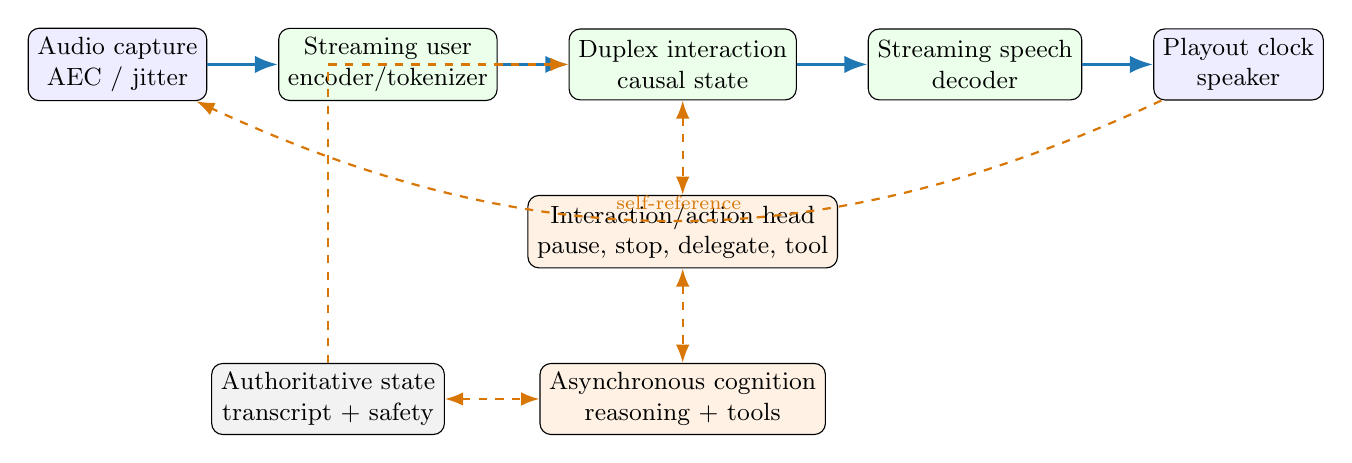
\begin{tikzpicture}[>=Latex,node distance=7mm and 9mm,font=\small,
box/.style={draw,rounded corners,align=center,minimum height=9mm},
f/.style={->,very thick,official},e/.style={->,thick,dashed,hypothesis}]
\node[box,fill=blue!7] (mic) {Audio capture\\AEC / jitter};
\node[box,fill=green!8,right=of mic] (enc) {Streaming user\\encoder/tokenizer};
\node[box,fill=green!8,right=of enc] (core) {Duplex interaction\\causal state};
\node[box,fill=green!8,right=of core] (dec) {Streaming speech\\decoder};
\node[box,fill=blue!7,right=of dec] (play) {Playout clock\\speaker};
\node[box,fill=orange!10,below=12mm of core] (action) {Interaction/action head\\pause, stop, delegate, tool};
\node[box,fill=orange!10,below=12mm of action] (frontier) {Asynchronous cognition\\reasoning + tools};
\node[box,fill=gray!10,left=12mm of frontier] (state) {Authoritative state\\transcript + safety};
\draw[f] (mic)--(enc); \draw[f] (enc)--(core); \draw[f] (core)--(dec); \draw[f] (dec)--(play);
\draw[e] (play) to[bend left=25] node[above,font=\scriptsize]{self-reference}(mic);
\draw[e,<->] (core)--(action); \draw[e,<->] (action)--(frontier); \draw[e,<->] (state)--(frontier); \draw[e] (state)|-(core);
\end{tikzpicture}%
}
\caption{可实现 GPT-Live 公开行为的最小架构重建。绿色语音内部结构与橙色动作头均属假设；官方确认的是持续交互、异步委派和系统边界。}
\label{zh:fig:reconstruction}
\end{figure}

\subsection{“混合架构”比“纯端到端”更准确}

在感知--发声路径上，端到端学习可以保留韵律、重叠和非语言信号；在复杂任务路径上，模块化委派允许使用更强推理模型、工具权限和独立扩缩容；在 transport/state 层，确定性协议和显式状态机仍不可替代。因此 GPT-Live 更像“端到端交互模型嵌入模块化实时系统”，而不是对所有组件做单模型吞并。

这种拆分还能带来安全和成本方面的优势：小而快的交互模型可以高频运行，昂贵模型只在必要时启动；工具权限集中在可审计的认知平面；安全控制可以同时作用于实时输出和后台结果。代价则是跨层一致性、过期结果处理、委派策略和会话状态恢复会更加复杂。

\section{一个可复现的开源实现方案}

\subsection{最小可行架构}

建议以三个独立服务实现研究原型：

\begin{enumerate}
  \item \textbf{Realtime gateway：}WebRTC ingress/egress、Opus、AEC/jitter buffer、播放时间戳、连接与弱网遥测。媒体包进入有界 ring buffer，应用事件进入可靠 data channel。
  \item \textbf{Duplex inference worker：}包括 causal audio encoder、文本 LLM backbone、user-stream adapter、assistant audio decoder 和 action head。worker 保持固定的 session affinity，每 80 或 160 ms 执行一次 inference tick。
  \item \textbf{Agent 与 state service：}负责最终转写、conversation event log、tool runtime、reasoning model、context compaction、安全策略和 instance handoff 协调。
\end{enumerate}

原型可以从 Moshi 开源栈的语音主干出发\cite{zh:defossez2024moshi}，增加独立的 action vocabulary 和 asynchronous tool bus；也可以采用 Freeze-Omni/LSLM 的路线，冻结文本 LLM，并接入 streaming encoder 和轻量 audio decoder，以降低训练成本\cite{zh:wang2024freezeomni,zh:ma2025lslm}。第一阶段不宜同时追求视频、超长 context 和多工具能力，应先验证真实 double-talk 条件下的 audio frame deadline 和打断行为。

\subsection{帧级调度伪代码}

\begin{algorithm}[H]
\caption{Deadline-aware duplex session loop}
\begin{algorithmic}[1]
\ForAll{active session $s$ in earliest-deadline order}
  \State $u_t\gets$ readAudioChunk$(s,\Delta)$
  \State $e_t\gets$ drainReadyEvents$(s,\mathrm{contextEpoch})$
  \State $(a_t,z_t,m_t)\gets$ duplexStep$(u_t,e_t,m_{t-1})$
  \If{$z_t$ requests delegation and no equivalent task is active}
    \State enqueueAsync$(taskId,\mathrm{contextEpoch},\mathrm{query})$
  \EndIf
  \If{safety permits $a_t$ and playout deadline remains}
    \State sendAudio$(s,a_t,\mathrm{timestamp})$
  \Else
    \State applyGracefulDegradation$(s)$
  \EndIf
\EndFor
\State run background prefill, compaction, and telemetry with residual budget
\end{algorithmic}
\end{algorithm}

调度循环需要避免三个隐蔽的阻塞点：tokenizer 或 audio codec 在 CPU 上串行执行；等待最终 ASR transcript 后才更新状态；在 media coroutine 中错误地同步等待 tool task。所有耗时操作都应通过 event 返回结果，media loop 只消费已经就绪的 event。

\subsection{分阶段实验计划}

\paragraph{阶段 A：离线可学习性。}
固定 7B--9B 文本 backbone 和 audio representation，在训练 token 数相同的条件下比较 channel fusion、cross-attention 和 gated fusion。训练集同时包含 half-duplex 对话、合成 overlap speech 和小规模真实双声道数据。验收标准包括：spoken QA 相对 half-duplex baseline 的退化不超过预设阈值；有效 barge-in 的 recall 提升且 false interruption rate 不恶化；存在 echo 时不发生 self-trigger。

\paragraph{阶段 B：单机实时性。}
在固定 GPU 上逐步增加并发 session，记录每个 tick 的 $Q/C$、DMR、P95/P99 jitter、KV cache 显存和 audio buffer underrun。比较 FIFO、continuous batching、earliest deadline first（EDF）以及预留 20\% 算力等策略。验收不以最高 token throughput 为准，而以每块 GPU 能稳定承载的 session 数为准。

\paragraph{阶段 C：异步认知。}
接入一个文本推理模型和三类工具：低延迟查询、长延迟搜索、多轮参数补全。对比不委派、阻塞式委派和异步委派三种模式，检查工具结果正确率、交互停顿、结果过期率、任务取消后的算力浪费，以及用户的主观等待感受。

\paragraph{阶段 D：长会话与故障。}
运行 30、60 和 120 分钟的长 session，主动注入 instance restart、network handoff、context compaction、transcript revision 和 tool-result race。验收标准包括：instance handoff 时不出现语音重复或缺失；context epoch 保持一致；用户关键事实得到保留；GPU 显存不随 session 时长无限增长。

\subsection{资源与延迟预算示例}

以 160 ms 为一个 inference tick 时，可以采用如下参考预算：uplink 与 jitter buffer 40 ms，streaming encoder 15 ms，interaction backbone 的 queueing 与 compute 45 ms，audio head 与 codec 20 ms，downlink、jitter buffer 和 playout 40 ms。这不是 GPT-Live 的公开参数，只是一个工程起点。预算必须使用 P95/P99 而不是平均值进行验证，并在跨地域、低端客户端和 5\% burst loss 条件下重新测试。

成本模型应按会话分钟分解为 interaction GPU、cognition GPU、音频带宽、tool 调用和 idle reservation。若委派率 $p_d$、平均 reasoning 时间 $T_r$、交互 core 每分钟成本 $C_f$，则粗略成本为
\begin{equation}
C_{min}=C_f+p_dT_rC_s+C_{net}+C_{tool}+C_{idle}.
\end{equation}
降低 $p_d$ 可以节省成本，但也可能损害任务正确率；因此，应结合委派准确率、召回率和最终任务成功率共同调优。

\section{局限性、开放问题与结论}

\subsection{仍然未知的关键细节}

本文不能回答 GPT-Live 的具体参数量、训练数据、codec、audio token rate、fusion 层位置、是否联合输出 action token、回声参考注入方式、推理并行策略和部署规模。这些信息从未被 OpenAI 官方公开。报告中的图~\ref{zh:fig:reconstruction} 是满足公开行为的\emph{一种最小实现}，不是泄露或反向工程结论。

现有论文之间也很难公平横比。Moshi 的“约 200 ms”、Neural-FSM 的“500 ms 内响应”、GPT-4o 的“平均 320 ms”使用不同任务、网络、硬件和延迟起点。本文保留这些数字用于说明各自设计目标，不把它们排成统一排行榜。

\subsection{研究前沿}

未来最值得关注的方向包括：（1）在强语义整合和抗 overlap 干扰之间，自适应地选择 user-stream routing；（2）将 speech、language 和 action 放在统一 clock 上，同时避免高频 acoustic token 淹没稀疏 action；（3）利用真实双声道数据训练能够适应不同文化 turn-taking 习惯的模型；（4）为长 session compaction 建立事实保真和可逆审计机制；（5）联合优化 inference tick、GPU scheduling、network jitter 和 playout clock；（6）建立覆盖 stale result、task cancellation 和 provenance tracking 的 asynchronous delegation benchmark。

\subsection{结论}

GPT-Live 的核心并不是某个神秘的声学模块，而是将语音智能体重构为持续运行的实时系统。与轮次式全模态模型相比，它允许新输入在生成期间持续进入模型状态，并让交互策略与现实时间同步；与早期的单模型全双工方案相比，它进一步把复杂认知任务放到异步路径中处理，并通过有状态推理服务、后台上下文压缩与实例切换、低往返时延 WebRTC，将模型能力转化为稳定的产品体验。

因此，复现 GPT-Live 不应从“训练一个更大的语音 LLM”开始，而应同时建立四个闭环：\textbf{表示闭环}保证说和听能够并行，\textbf{控制闭环}学习停顿与打断，\textbf{认知闭环}安全地执行异步委派，\textbf{系统闭环}确保每个音频帧都能在播放时限之前到达。公开论文已经给出了这些组件的大部分候选机制；真正困难、也最有研究价值的，是让它们在同一个在线系统中稳定协同。

{\footnotesize
\begin{thebibliography}{38}
\providecommand{\natexlab}[1]{#1}
\providecommand{\url}[1]{\texttt{#1}}
\expandafter\ifx\csname urlstyle\endcsname\relax
  \providecommand{\doi}[1]{doi: #1}\else
  \providecommand{\doi}{doi: \begingroup \urlstyle{rm}\Url}\fi

\bibitem[{OpenAI}(2026{\natexlab{a}})]{zh:openai2026continuous}
{OpenAI}.
\newblock How we built a realtime system for responsive voice {AI} in six
  months, August 2026{\natexlab{a}}.
\newblock URL
  \url{https://openai.com/index/continuous-voice-interaction-with-gpt-live/}.
\newblock Accessed 2026-08-07.

\bibitem[{OpenAI}(2026{\natexlab{b}})]{zh:openai2026gptlive}
{OpenAI}.
\newblock Introducing {GPT-Live}, August 2026{\natexlab{b}}.
\newblock URL \url{https://openai.com/index/introducing-gpt-live/}.
\newblock Accessed 2026-08-07.

\bibitem[{OpenAI}(2024)]{zh:openai2024gpt4osystemcard}
{OpenAI}.
\newblock {GPT-4o} system card, August 2024.
\newblock URL \url{https://openai.com/index/gpt-4o-system-card/}.
\newblock Accessed 2026-08-07.

\bibitem[Xu et~al.(2025)Xu, Guo, He, Hu, He, Bai, Chen, Wang, Fan, Dang, Zhang,
  Wang, Chu, and Lin]{zh:xu2025qwenomni}
Jin Xu, Zhifang Guo, Jinzheng He, Hangrui Hu, Ting He, Shuai Bai, Keqin Chen,
  Jialin Wang, Yang Fan, Kai Dang, Bin Zhang, Xiong Wang, Yunfei Chu, and
  Junyang Lin.
\newblock {Qwen2.5-Omni} technical report.
\newblock \emph{arXiv preprint arXiv:2503.20215}, 2025.
\newblock URL \url{https://arxiv.org/abs/2503.20215}.

\bibitem[Zeng et~al.(2024)Zeng, Du, Liu, Wang, Jiang, Zhao, Dong, and
  Tang]{zh:zeng2024glm4voice}
Aohan Zeng, Zhengxiao Du, Mingdao Liu, Kedong Wang, Shengmin Jiang, Lei Zhao,
  Yuxiao Dong, and Jie Tang.
\newblock {GLM-4-Voice}: Towards intelligent and human-like end-to-end spoken
  chatbot.
\newblock \emph{arXiv preprint arXiv:2412.02612}, 2024.
\newblock URL \url{https://arxiv.org/abs/2412.02612}.

\bibitem[Xie and Wu(2024)]{zh:xie2024miniomni}
Zhifei Xie and Changqiao Wu.
\newblock Mini-omni: Language models can hear, talk while thinking in
  streaming.
\newblock \emph{arXiv preprint arXiv:2408.16725}, 2024.
\newblock URL \url{https://arxiv.org/abs/2408.16725}.

\bibitem[D{\'e}fossez et~al.(2024)D{\'e}fossez, Mazar{\'e}, Orsini, Royer,
  P{\'e}rez, J{\'e}gou, Grave, and Zeghidour]{zh:defossez2024moshi}
Alexandre D{\'e}fossez, Laurent Mazar{\'e}, Manu Orsini, Am{\'e}lie Royer,
  Patrick P{\'e}rez, Herv{\'e} J{\'e}gou, Edouard Grave, and Neil Zeghidour.
\newblock Moshi: A speech-text foundation model for real-time dialogue.
\newblock \emph{arXiv preprint arXiv:2410.00037}, 2024.
\newblock URL \url{https://arxiv.org/abs/2410.00037}.

\bibitem[Veluri et~al.(2024)Veluri, Peloquin, Yu, Gong, and
  Gollakota]{zh:veluri2024syncllm}
Bandhav Veluri, Benjamin~N. Peloquin, Bokai Yu, Hongyu Gong, and Shyamnath
  Gollakota.
\newblock Beyond turn-based interfaces: Synchronous {LLM}s as full-duplex
  dialogue agents.
\newblock In \emph{Proceedings of EMNLP}, pages 21390--21402, 2024.
\newblock \doi{10.18653/v1/2024.emnlp-main.1192}.
\newblock URL \url{https://aclanthology.org/2024.emnlp-main.1192/}.

\bibitem[Ma et~al.(2025)Ma, Song, Du, Cong, Chen, Wang, Wang, and
  Chen]{zh:ma2025lslm}
Ziyang Ma, Yakun Song, Chenpeng Du, Jian Cong, Zhuo Chen, Yuping Wang, Yuxuan
  Wang, and Xie Chen.
\newblock Language model can listen while speaking.
\newblock In \emph{Proceedings of the AAAI Conference on Artificial
  Intelligence}, 2025.
\newblock URL \url{https://arxiv.org/abs/2408.02622}.

\bibitem[Wang et~al.(2024{\natexlab{a}})Wang, Lu, Tang, Yan, Xia, and
  Xiong]{zh:wang2024neuralfsm}
Peng Wang, Songshuo Lu, Yaohua Tang, Sijie Yan, Wei Xia, and Yuanjun Xiong.
\newblock A full-duplex speech dialogue scheme based on large language model.
\newblock In \emph{Advances in Neural Information Processing Systems},
  volume~37, 2024{\natexlab{a}}.
\newblock URL
  \url{https://proceedings.neurips.cc/paper_files/paper/2024/hash/180d4373aca26bd86bf45fc50d1a709f-Abstract-Conference.html}.

\bibitem[Huang et~al.(2026)Huang, Zhang, Yu, Shi, Ma, Xu, Gao, Hao, He, and
  Liu]{zh:huang2026duplexomni}
Muye Huang, Lingling Zhang, Xingyu Yu, Lei Shi, Zhanyu Ma, Jun Xu, Jiuchong
  Gao, Jinghua Hao, Renqing He, and Jun Liu.
\newblock Duplexomni: Real-time listening, seeing, thinking, and speaking for
  full-duplex interaction.
\newblock \emph{arXiv preprint arXiv:2606.09186}, 2026.
\newblock URL \url{https://arxiv.org/abs/2606.09186}.

\bibitem[{OpenAI}(2026{\natexlab{c}})]{zh:openai2026safety}
{OpenAI}.
\newblock {GPT-Live} system card, August 2026{\natexlab{c}}.
\newblock URL \url{https://deploymentsafety.openai.com/gpt-live}.
\newblock Accessed 2026-08-07.

\bibitem[Vaswani et~al.(2017)Vaswani, Shazeer, Parmar, Uszkoreit, Jones, Gomez,
  Kaiser, and Polosukhin]{zh:vaswani2017attention}
Ashish Vaswani, Noam Shazeer, Niki Parmar, Jakob Uszkoreit, Llion Jones,
  Aidan~N. Gomez, Lukasz Kaiser, and Illia Polosukhin.
\newblock Attention is all you need.
\newblock In \emph{Advances in Neural Information Processing Systems},
  volume~30, 2017.
\newblock URL \url{https://arxiv.org/abs/1706.03762}.

\bibitem[Zhang et~al.(2026)Zhang, Chen, Wu, Li, Zhang, Zhang, Liu, Lin, Peng,
  Liu, Chng, Yan, Wu, Huang, Yang, and Tian]{zh:zhang2026duplexsla}
Haoyang Zhang, Jun Chen, Donghang Wu, Yuxin Li, Yuxin Zhang, Xiangyu~Tony
  Zhang, Che Liu, Qingjian Lin, Yizhou Peng, Hexin Liu, Eng~Siong Chng, Chao
  Yan, Boyong Wu, Yechang Huang, Xuerui Yang, and Fei Tian.
\newblock Duplexsla: A full-duplex spoken language model with synchronized
  speech, language, and action.
\newblock \emph{arXiv preprint arXiv:2605.20755}, 2026.
\newblock URL \url{https://arxiv.org/abs/2605.20755}.

\bibitem[Yu et~al.(2025)Yu, Wang, Yang, Chen, Tian, Zhang, Sun, Lu, Wang, and
  Zhang]{zh:yu2025salmonnomni}
Wenyi Yu, Siyin Wang, Xiaoyu Yang, Xianzhao Chen, Xiaohai Tian, Jun Zhang,
  Guangzhi Sun, Lu~Lu, Yuxuan Wang, and Chao Zhang.
\newblock {SALMONN}-omni: A standalone speech {LLM} without codec injection for
  full-duplex conversation.
\newblock In \emph{Advances in Neural Information Processing Systems},
  volume~38, 2025.
\newblock URL
  \url{https://proceedings.neurips.cc/paper_files/paper/2025/hash/233aee920dab065709145371b5900b8f-Abstract-Conference.html}.

\bibitem[Zeghidour et~al.(2022)Zeghidour, Luebs, Omran, Skoglund, and
  Tagliasacchi]{zh:zeghidour2021soundstream}
Neil Zeghidour, Alejandro Luebs, Ahmed Omran, Jan Skoglund, and Marco
  Tagliasacchi.
\newblock Soundstream: An end-to-end neural audio codec.
\newblock \emph{IEEE/ACM Transactions on Audio, Speech, and Language
  Processing}, 30:\penalty0 495--507, 2022.
\newblock URL \url{https://arxiv.org/abs/2107.03312}.

\bibitem[D{\'e}fossez et~al.(2022)D{\'e}fossez, Copet, Synnaeve, and
  Adi]{zh:defossez2022encodec}
Alexandre D{\'e}fossez, Jade Copet, Gabriel Synnaeve, and Yossi Adi.
\newblock High fidelity neural audio compression.
\newblock \emph{arXiv preprint arXiv:2210.13438}, 2022.
\newblock URL \url{https://arxiv.org/abs/2210.13438}.

\bibitem[Borsos et~al.(2022)Borsos, Marinier, Vincent, Kharitonov, Pietquin,
  Sharifi, Roblek, Teboul, Grangier, Tagliasacchi, and
  Zeghidour]{zh:borsos2022audiolm}
Zal{\'a}n Borsos, Rapha{\"e}l Marinier, Damien Vincent, Eugene Kharitonov,
  Olivier Pietquin, Matt Sharifi, Dominik Roblek, Olivier Teboul, David
  Grangier, Marco Tagliasacchi, and Neil Zeghidour.
\newblock {AudioLM}: A language modeling approach to audio generation.
\newblock \emph{arXiv preprint arXiv:2209.03143}, 2022.
\newblock URL \url{https://arxiv.org/abs/2209.03143}.

\bibitem[Long et~al.(2025)Long, Shen, Fu, Gao, Li, Chen, Zhang, Shao, Li, Peng,
  Cao, Li, Ji, and Sun]{zh:long2025vitaaudio}
Zuwei Long, Yunhang Shen, Chaoyou Fu, Heting Gao, Lijiang Li, Peixian Chen,
  Mengdan Zhang, Hang Shao, Jian Li, Jinlong Peng, Haoyu Cao, Ke~Li, Rongrong
  Ji, and Xing Sun.
\newblock {VITA-Audio}: Fast interleaved cross-modal token generation for
  efficient large speech-language model.
\newblock \emph{arXiv preprint arXiv:2505.03739}, 2025.
\newblock URL \url{https://arxiv.org/abs/2505.03739}.

\bibitem[Chen and Yu(2025)]{zh:chen2025survey}
Yuxuan Chen and Haoyuan Yu.
\newblock From turn-taking to synchronous dialogue: A survey of full-duplex
  spoken language models.
\newblock \emph{arXiv preprint arXiv:2509.14515}, 2025.
\newblock URL \url{https://arxiv.org/abs/2509.14515}.

\bibitem[Zhang et~al.(2024)Zhang, Cheng, Deng, Chen, Wang, Zheng, Liu, Yu, Tan,
  Du, and Zhang]{zh:zhang2024omniflatten}
Qinglin Zhang, Luyao Cheng, Chong Deng, Qian Chen, Wen Wang, Siqi Zheng,
  Jiaqing Liu, Hai Yu, Chaohong Tan, Zhihao Du, and Shiliang Zhang.
\newblock Omniflatten: An end-to-end {GPT} model for seamless voice
  conversation.
\newblock \emph{arXiv preprint arXiv:2410.17799}, 2024.
\newblock URL \url{https://arxiv.org/abs/2410.17799}.

\bibitem[Nguyen et~al.(2022)Nguyen, Kharitonov, Copet, Adi, Hsu, Elkahky,
  Tomasello, Algayres, Sagot, Mohamed, and Dupoux]{zh:nguyen2022dgslm}
Tu~Anh Nguyen, Eugene Kharitonov, Jade Copet, Yossi Adi, Wei-Ning Hsu, Ali
  Elkahky, Paden Tomasello, Robin Algayres, Benoit Sagot, Abdelrahman Mohamed,
  and Emmanuel Dupoux.
\newblock Generative spoken dialogue language modeling.
\newblock \emph{arXiv preprint arXiv:2203.16502}, 2022.
\newblock URL \url{https://arxiv.org/abs/2203.16502}.

\bibitem[Lu et~al.(2026)Lu, Chen, Wang, Peng, Kang, Wu, and Wu]{zh:lu2026routing}
Hui Lu, Xueyuan Chen, Huimeng Wang, Shuhai Peng, Shiyin Kang, Xixin Wu, and
  Zhiyong Wu.
\newblock How should {LLM}s listen while speaking? a study of user-stream
  routing in full-duplex spoken dialogue.
\newblock \emph{arXiv preprint arXiv:2605.10199}, 2026.
\newblock URL \url{https://arxiv.org/abs/2605.10199}.

\bibitem[Nakata et~al.(2026)Nakata, Saito, and
  Saruwatari]{zh:nakata2026duplexchat}
Wataru Nakata, Yuki Saito, and Hiroshi Saruwatari.
\newblock Duplexchat: Constructing speaker-separated full-duplex dialogue
  speech at scale for spoken dialogue language modeling.
\newblock \emph{arXiv preprint arXiv:2607.04941}, 2026.
\newblock URL \url{https://arxiv.org/abs/2607.04941}.

\bibitem[Wang et~al.(2024{\natexlab{b}})Wang, Li, Fu, Shen, Xie, Li, Sun, and
  Ma]{zh:wang2024freezeomni}
Xiong Wang, Yangze Li, Chaoyou Fu, Yunhang Shen, Lei Xie, Ke~Li, Xing Sun, and
  Long Ma.
\newblock Freeze-omni: A smart and low latency speech-to-speech dialogue model
  with frozen {LLM}.
\newblock \emph{arXiv preprint arXiv:2411.00774}, 2024{\natexlab{b}}.
\newblock URL \url{https://arxiv.org/abs/2411.00774}.

\bibitem[Dai et~al.(2019)Dai, Yang, Yang, Carbonell, Le, and
  Salakhutdinov]{zh:dai2019transformerxl}
Zihang Dai, Zhilin Yang, Yiming Yang, Jaime Carbonell, Quoc~V. Le, and Ruslan
  Salakhutdinov.
\newblock Transformer-{XL}: Attentive language models beyond a fixed-length
  context.
\newblock \emph{arXiv preprint arXiv:1901.02860}, 2019.
\newblock URL \url{https://arxiv.org/abs/1901.02860}.

\bibitem[Kwon et~al.(2023)Kwon, Li, Zhuang, Sheng, Zheng, Yu, Gonzalez, Zhang,
  and Stoica]{zh:kwon2023pagedattention}
Woosuk Kwon, Zhuohan Li, Siyuan Zhuang, Ying Sheng, Lianmin Zheng, Cody~Hao Yu,
  Joseph~E. Gonzalez, Hao Zhang, and Ion Stoica.
\newblock Efficient memory management for large language model serving with
  {PagedAttention}.
\newblock In \emph{Proceedings of the ACM Symposium on Operating Systems
  Principles}, 2023.
\newblock URL \url{https://arxiv.org/abs/2309.06180}.

\bibitem[Dao et~al.(2022)Dao, Fu, Ermon, Rudra, and
  R{\'e}]{zh:dao2022flashattention}
Tri Dao, Daniel~Y. Fu, Stefano Ermon, Atri Rudra, and Christopher R{\'e}.
\newblock {FlashAttention}: Fast and memory-efficient exact attention with
  {IO}-awareness.
\newblock In \emph{Advances in Neural Information Processing Systems},
  volume~35, 2022.
\newblock URL \url{https://arxiv.org/abs/2205.14135}.

\bibitem[Leviathan et~al.(2023)Leviathan, Kalman, and
  Matias]{zh:leviathan2023speculative}
Yaniv Leviathan, Matan Kalman, and Yossi Matias.
\newblock Fast inference from transformers via speculative decoding.
\newblock In \emph{Proceedings of ICML}, 2023.
\newblock URL \url{https://arxiv.org/abs/2211.17192}.

\bibitem[Alvestrand(2021)]{zh:alvestrand2021webrtc}
Harald Alvestrand.
\newblock Overview: Real-time protocols for browser-based applications.
\newblock Technical Report RFC 8825, Internet Engineering Task Force, 2021.
\newblock URL \url{https://datatracker.ietf.org/doc/rfc8825/}.

\bibitem[Jesup et~al.(2021)Jesup, Loreto, and T{\"u}xen]{zh:jesup2021datachannels}
Randell Jesup, Salvatore Loreto, and Michael T{\"u}xen.
\newblock {WebRTC} data channels.
\newblock Technical Report RFC 8831, Internet Engineering Task Force, 2021.
\newblock URL \url{https://datatracker.ietf.org/doc/rfc8831/}.

\bibitem[Agranovich et~al.(2024)Agranovich, Nachmani, Rybakov, Ding, Jia, Bar,
  Zen, and Ramanovich]{zh:agranovich2024simultron}
Alex Agranovich, Eliya Nachmani, Oleg Rybakov, Yifan Ding, Ye~Jia, Nadav Bar,
  Heiga Zen, and Michelle~Tadmor Ramanovich.
\newblock Simultron: On-device simultaneous speech-to-speech translation.
\newblock \emph{arXiv preprint arXiv:2406.02133}, 2024.
\newblock URL \url{https://arxiv.org/abs/2406.02133}.

\bibitem[Rescorla et~al.(2022)Rescorla, Tschofenig, and
  Modadugu]{zh:rescorla2022dtls13}
Eric Rescorla, Hannes Tschofenig, and Nagendra Modadugu.
\newblock The datagram transport layer security ({DTLS}) protocol version 1.3.
\newblock Technical Report RFC 9147, Internet Engineering Task Force, 2022.
\newblock URL \url{https://datatracker.ietf.org/doc/rfc9147/}.

\bibitem[Hancke et~al.(2026)Hancke, Rescorla, and Rose]{zh:hancke2026sped}
Philipp Hancke, Eric Rescorla, and Jonny Rose.
\newblock {SPED}: {STUN} protocol for embedding {DTLS}.
\newblock Technical Report draft-hancke-webrtc-sped-00, Internet Engineering
  Task Force, 2026.
\newblock URL \url{https://datatracker.ietf.org/doc/draft-hancke-webrtc-sped/}.
\newblock Internet-Draft, work in progress.

\bibitem[Hancke and Rescorla(2026)]{zh:hancke2026snap}
Philipp Hancke and Eric Rescorla.
\newblock {SNAP}: Accelerating {WebRTC} data channel establishment.
\newblock Technical Report draft-hancke-tsvwg-snap-00, Internet Engineering
  Task Force, 2026.
\newblock URL \url{https://datatracker.ietf.org/doc/draft-hancke-tsvwg-snap/}.
\newblock Internet-Draft, work in progress.

\bibitem[Lin et~al.(2025)Lin, Lian, Li, Wang, Anumanchipalli, Liu, and
  Lee]{zh:lin2025fullduplexbench}
Guan-Ting Lin, Jiachen Lian, Tingle Li, Qirui Wang, Gopala Anumanchipalli,
  Alexander~H. Liu, and Hung-yi Lee.
\newblock Full-duplex-bench: A benchmark to evaluate full-duplex spoken
  dialogue models on turn-taking capabilities.
\newblock \emph{arXiv preprint arXiv:2503.04721}, 2025.
\newblock URL \url{https://arxiv.org/abs/2503.04721}.

\bibitem[Lin et~al.(2026)Lin, Kuan, Shi, Chang, Arora, Watanabe, and
  Lee]{zh:lin2026fullduplexbenchv2}
Guan-Ting Lin, Shih-Yun~Shan Kuan, Jiatong Shi, Kai-Wei Chang, Siddhant Arora,
  Shinji Watanabe, and Hung-yi Lee.
\newblock Full-duplex-bench-v2: A multi-turn evaluation framework for duplex
  dialogue systems with an automated examiner.
\newblock In \emph{Proceedings of ACL}, 2026.
\newblock URL \url{https://aclanthology.org/2026.acl-short.4/}.

\bibitem[Stivers et~al.(2009)Stivers, Enfield, Brown, Englert, Hayashi,
  Heinemann, Hoymann, Rossano, de~Ruiter, Yoon, and
  Levinson]{zh:stivers2009turntaking}
Tanya Stivers, N.~J. Enfield, Penelope Brown, Christina Englert, Makoto
  Hayashi, Trine Heinemann, Gertie Hoymann, Federico Rossano, Jan~Peter
  de~Ruiter, Kyung-Eun Yoon, and Stephen~C. Levinson.
\newblock Universals and cultural variation in turn-taking in conversation.
\newblock \emph{Proceedings of the National Academy of Sciences}, 106\penalty0
  (26):\penalty0 10587--10592, 2009.
\newblock \doi{10.1073/pnas.0903616106}.

\end{thebibliography}
}
\end{document}
